\documentclass[12pt]{article}
\usepackage{amsmath}
\usepackage{graphicx}
\usepackage{adjustbox}
\usepackage{booktabs}
\usepackage{tabularx}
\usepackage{fullpage}
\usepackage{subcaption}
\usepackage{cite}
\usepackage{float} % Added to allow [H] float specifier



\title{Spatio-Temporal Machine Learning for Economic Forecasting: A Cross-Indicator and Cross-Country Analysis Using World Bank Data}
\author{Jiadong Zhang\thanks{Email: \texttt{dereksodo@gmail.com}}}
\date{May 2025}

\begin{document}

\maketitle

\begin{abstract}
This paper develops a spatio-temporal framework for forecasting key macroeconomic indicators using machine learning techniques. Leveraging World Bank panel data from 1960 to 2020, we investigate three core tasks: (1) cross-indicator prediction—forecasting one major indicator based on others; (2) national-level time series forecasting; and (3) cross-national forecasting for major economies. Through comparative analysis of models including XGBoost, Random Forest, and linear baselines, we find that most structural indicators are highly predictable, while GDP growth remains volatile and difficult to model. We introduce a novel feasibility rate metric to assess reliability across multiple performance dimensions. Our results highlight both the promise and the limitations of data-driven methods in economic forecasting and underscore the importance of model selection, data context, and indicator stability.
\end{abstract}

\newpage
\tableofcontents
\newpage


\section{Introduction}

Macroeconomic indicators provide a comprehensive lens for assessing the economic and social development of countries. This study leverages World Bank panel data from 1960 to 2020 to identify key national indicators and evaluate their predictability using machine learning. The focus is on cross-indicator prediction: can one major indicator be reliably predicted from the others?
\section{Literature Review}

Recent advancements in machine learning (ML) have significantly influenced macroeconomic forecasting. This section reviews key studies that have explored the integration of ML techniques into economic prediction models.

\subsection{Nonlinearity and Regularization in ML Forecasting}

Goulet Coulombe et al. (2019) investigate the efficacy of ML in macroeconomic forecasting, emphasizing the importance of capturing nonlinear relationships in economic data. Their study concludes that nonlinearity is a crucial factor in improving forecast accuracy. They also highlight that traditional factor models serve as effective regularization tools within ML frameworks, aiding in managing model complexity and preventing overfitting. The authors advocate for the use of K-fold cross-validation as a best practice for model evaluation and selection. Their findings suggest that ML models, when properly regularized and validated, can outperform traditional econometric models, especially during periods of economic uncertainty and financial stress \cite{GouletCoulombe2019}.

\subsection{Automating Forecasting with ML Techniques}

Hall (2018) explores the application of ML methods to macroeconomic forecasting, focusing on the automation of model selection and parameter tuning. The study demonstrates that ML algorithms can process vast and complex datasets, identifying patterns that traditional models might overlook. Hall's analysis reveals that ML models can outperform both simple time-series models and consensus forecasts from professional economists, particularly in predicting short-term economic indicators like the unemployment rate. The research underscores the potential of ML to enhance forecasting accuracy by reducing reliance on manual model specification and expert judgment \cite{Hall2018}.

\subsection{ML Applications in China's GDP Forecasting}

Yang et al. (2024) apply various ML models to forecast China's quarterly real GDP growth, assessing their performance against traditional econometric models and expert forecasts. Their study finds that ML models generally achieve lower forecast errors, particularly during stable economic periods. However, during economic inflection points, expert forecasts may exhibit greater accuracy due to a more nuanced understanding of the macroeconomic environment. Additionally, the authors employ interpretable ML techniques to identify key variables influencing GDP fluctuations, providing insights into the underlying drivers of economic change \cite{Yang2024}.

\subsection{Synthesis and Implications for Current Research}

The reviewed studies collectively highlight the transformative impact of ML on macroeconomic forecasting. They demonstrate that ML models, with their ability to capture complex nonlinear relationships and process large datasets, can enhance forecast accuracy beyond traditional methods. These findings inform the current research by underscoring the importance of incorporating ML techniques into economic prediction models, particularly for analyzing cross-indicator relationships, time series data, and cross-country economic dynamics.
While the empirical studies reviewed above emphasize the technical advances of ML-based forecasting, it is equally important to align these findings with economic theory. For instance, the persistent unpredictability of GDP growth observed in both past studies and our own results echoes theoretical insights from the Solow growth model\cite{Solow1956}, which attributes long-term economic growth primarily to exogenous technological progress—a factor that is inherently difficult to observe or predict. Likewise, indicators such as life expectancy and energy consumption—which consistently achieve low RMSE/STD and MASE and high $R^2$ and DA—reflect long-term structural trends that are more stable and easier to model. The declining predictive value of agricultural output aligns with structural transformation theory, which explains the shift of economic activity from agriculture to industry and services as economies develop. By framing ML findings within established theoretical paradigms, this study highlights not only algorithmic performance but also its macroeconomic interpretability.\cite{Solow1956, Kuznets1971}

% This section should review key literature on macroeconomic forecasting using machine learning.
% Include comparisons of cross-indicator modeling, single-country time series forecasting, and international panel data approaches.
% Discuss how your work extends or differs from past studies such as Goulet Coulombe (2019), Hall (2018), and Yang et al. (2024).
\section{Data and Methods}

\subsection{Data Source}

\begin{itemize}
    \item World Bank Open Data, 1960--2020, including G20 expect African Union.
    \item Main dataset: [World Bank Data by Indicators](https://github.com/light-and-salt/World-Bank-Data-by-Indicators) (GitHub repository)
    \item We selected features with more than 60\% of relevant data present to minimize interpolation errors, resulting in a subset of 13 indicators. From these, we identified 10 relatively independent features for modeling, denoted $\{F_1, F_2, \ldots, F_{10}\}$.\footnote{Check Table \ref{tab:indicator_table} for details.}
\end{itemize}

\begin{table}[H]
    \centering
    \small
    \adjustbox{center}{
        \begin{tabular}{|c|c|}
            \hline
            \textbf{Indicator Code} & \textbf{Indicator Name} \\
            \hline
            SP.DYN.LE00.IN & Life expectancy at birth, total (years) \\
            SP.URB.TOTL.IN.ZS & Urban population (\% of total population) \\
            NV.AGR.TOTL.ZS & Agriculture, forestry, and fishing, value added (\% of GDP) \\
            EG.USE.PCAP.KG.OE & Energy use (kg of oil equivalent per capita) \\
            FS.AST.PRVT.GD.ZS & Assets of private sector banks to GDP (\%) \\
            NE.IMP.GNFS.ZS & Imports of goods and services (\% of GDP) \\
            NY.GDP.MKTP.CD & GDP (current US\$) \\
            NE.EXP.GNFS.ZS & Exports of goods and services (\% of GDP) \\
            NY.GDP.MKTP.KD.ZG & GDP growth (annual \%) \\
            EN.ATM.GHGT.KT.CE & Total greenhouse gas emissions (kt of CO$_2$  equivalent) \\
            \hline
        \end{tabular}
    }
    \caption{Indicator Table}
    \label{tab:indicator_table}
\end{table}

\subsection{Data Preprocessing}

\begin{itemize}
    \item Interpolated missing values for convenience.
    \item Constructed a country-year-feature panel: each row is a unique (country, year) pair.
\end{itemize}



\subsection{Machine Learning Models}

The following models are compared\footnote{See /src/DataProcessing/models.py for parameters}:
\begin{itemize}
    \item Linear Regression (LR)
    \item Ridge Regression
    \item Lasso Regression
    \item Elastic Net
    \item Support Vector Regression (SVR)
    \item Random Forest (RF)
    \item K-Nearest Neighbors (KNN)
    \item XGBoost
    \item Locally Weighted Regression (LWR)
\end{itemize}

\subsection{Experimental Setup}

\begin{itemize}
    \item \textbf{Year ranges:}
    \begin{itemize}
        \item Full period: 1960--2020
        \item Recent period: 2010--2020
    \end{itemize}
    \item \textbf{Cross-Validation:} 5-fold cross-validation is used for each prediction, averaging metrics across folds.
    \item \textbf{Evaluation Metrics:}
    \begin{itemize}
        \item Standardized error (RMSE/STD)~\cite{ChaiDraxler2014}, threshold = 1
        \item Coefficient of Determination ($R^2$)~\cite{Alexander2001}, threshold = 0.6
        \item Mean Absolute Scaled Error (MASE)~\cite{Hyndman2006}, threshold = 1
        \item Directional Accuracy (DA)~\cite{Hyndman2006}, threshold = 0.7
        \item \textbf{Guiding Metric (Heuristic Indicator):} For each model and indicator, we define a guiding metric score as the weighted score consisting of 4 metircs. Specifically, we compute:
        \begin{align*}
        \alpha_1 &= -\frac{\frac{\text{RMSE}_i}{\text{STD}_i} - 1}{1} \\\\
        \alpha_2 &= \frac{R_i^2 - 0.6}{0.6} \\\\
        \alpha_3 &= -\frac{\text{MASE}_i - 1}{1} \\\\
        \alpha_4 &= \frac{\text{DA}_i - 0.7}{0.7}
        \end{align*}
        \[
        \text{Guiding Score} = \sum_{i=1}^4 \frac{\beta_i}{1 + \exp(-\alpha_i)}
        \]
        $\beta_i$ is the weight assigned to each standard metric, and in this paper we choose $\beta = \{2.0, 2.0, 1.0, 5.0\}$ because when making policies the direction seems more important than the actual value. When all metrics are at their thresholds, Guiding Score = 2.0, also the threshold for Guiding Metric.
    \end{itemize}
    \item \textbf{Visualization:} For each model and year range, bar plots of the metrics are generated, with feasible region thresholds indicated.
\end{itemize}

\section{Cross-Indicator Forecasting}

\subsection{Prediction Task}
For each indicator $F_k$, we predict its value for each country-year using the remaining 9 indicators as input features. The process is repeated for all $k = 1, \ldots, 10$.
\subsection{Prediction Results}
% Retain your current performance evaluation here.

% Sample Figure Placeholders
\begin{figure}[h]
    \centering
    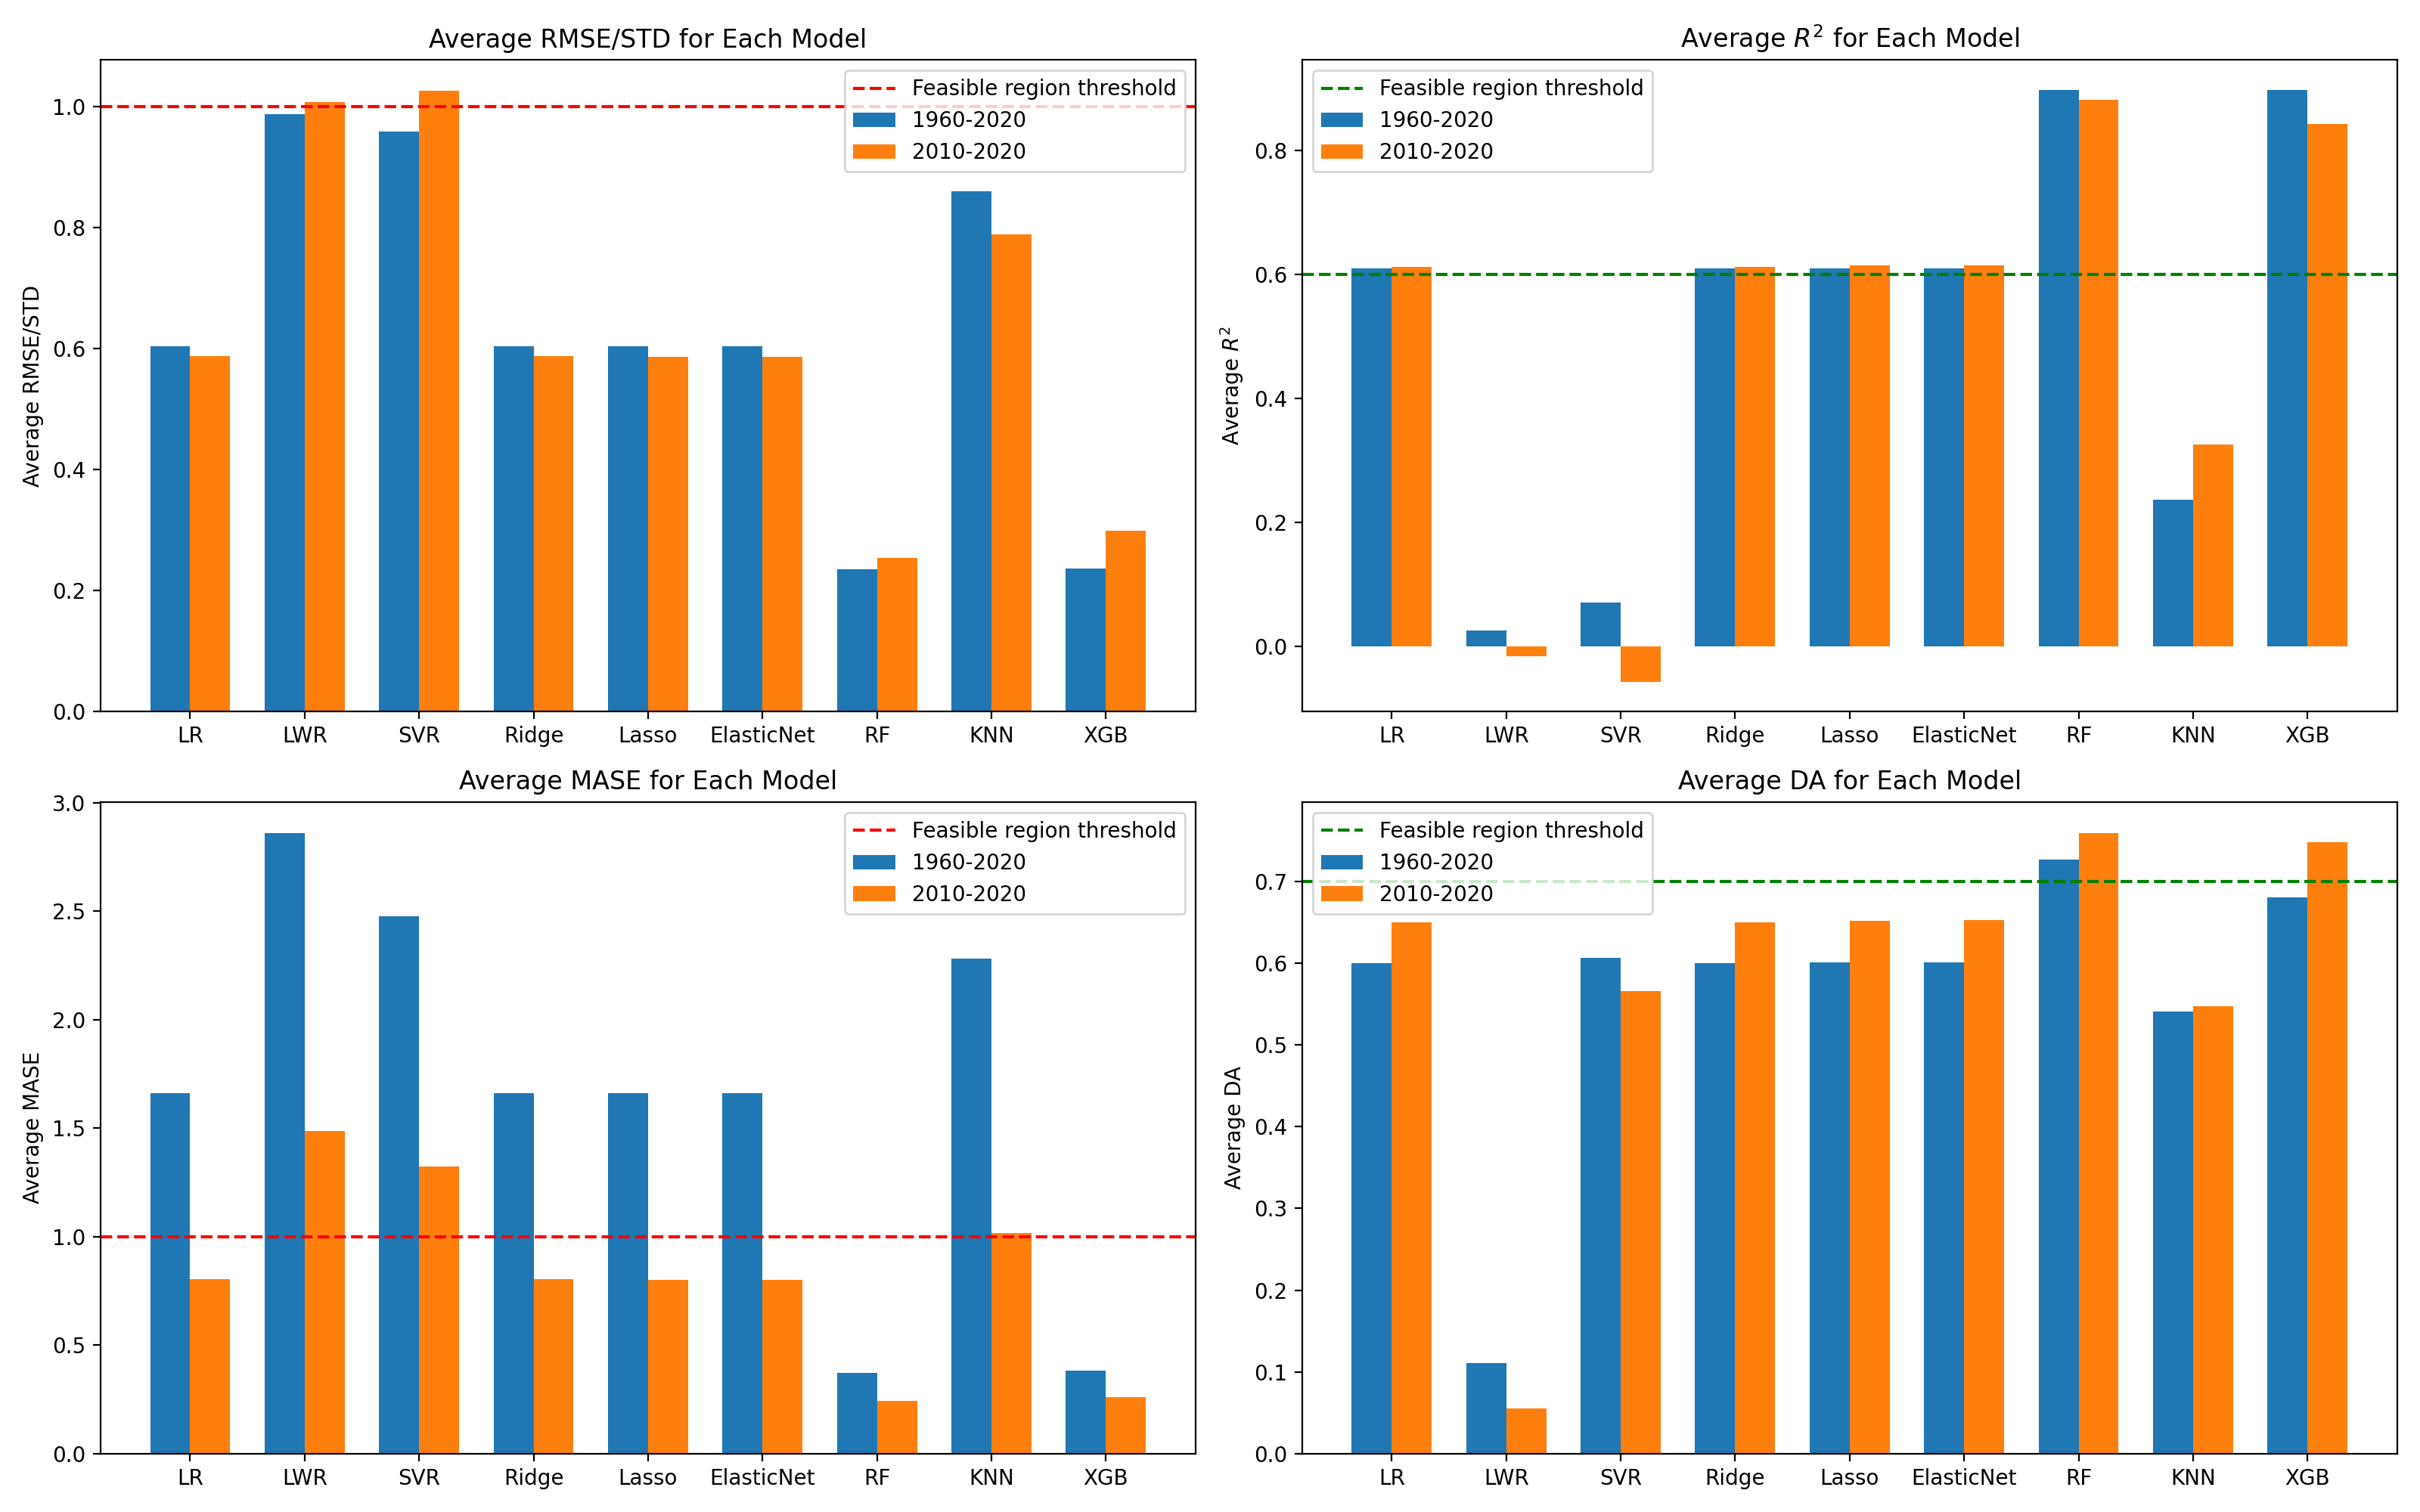
\includegraphics[width = \linewidth]{Combined_Metrics_figure1.png}
    
    \caption{Comparison of Model Performance: RMSE/STD, $R^2$, MASE and DA (1960–2020, 2010–2020)}
    \label{fig:model_compare_1}
\end{figure}
\begin{figure}[H]
    \centering
    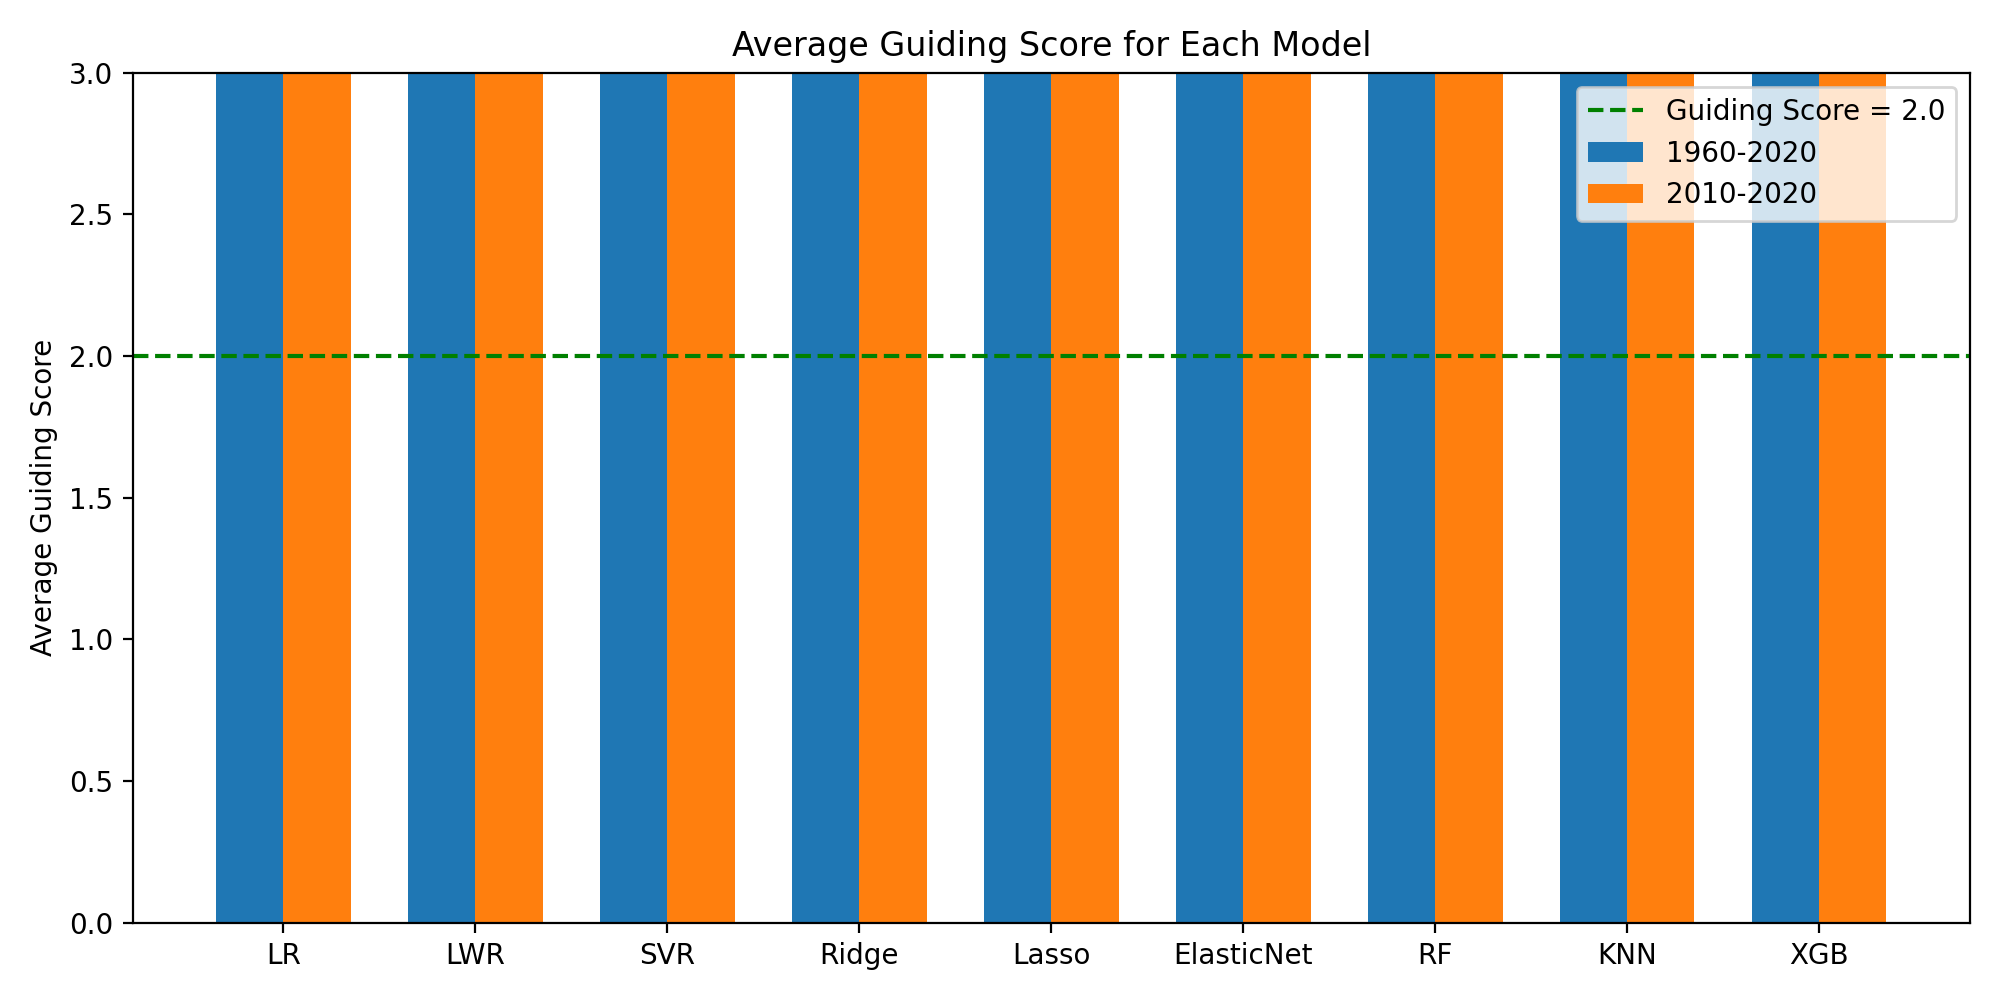
\includegraphics[width = \linewidth]{Average_GuidingScore_figure2.png}
    \caption{Comparison of Model Performance: Guiding Score (1960–2020, 2010–2020)}
    \label{fig:model_compare_2}
\end{figure}
\begin{figure}[H]
    \centering
    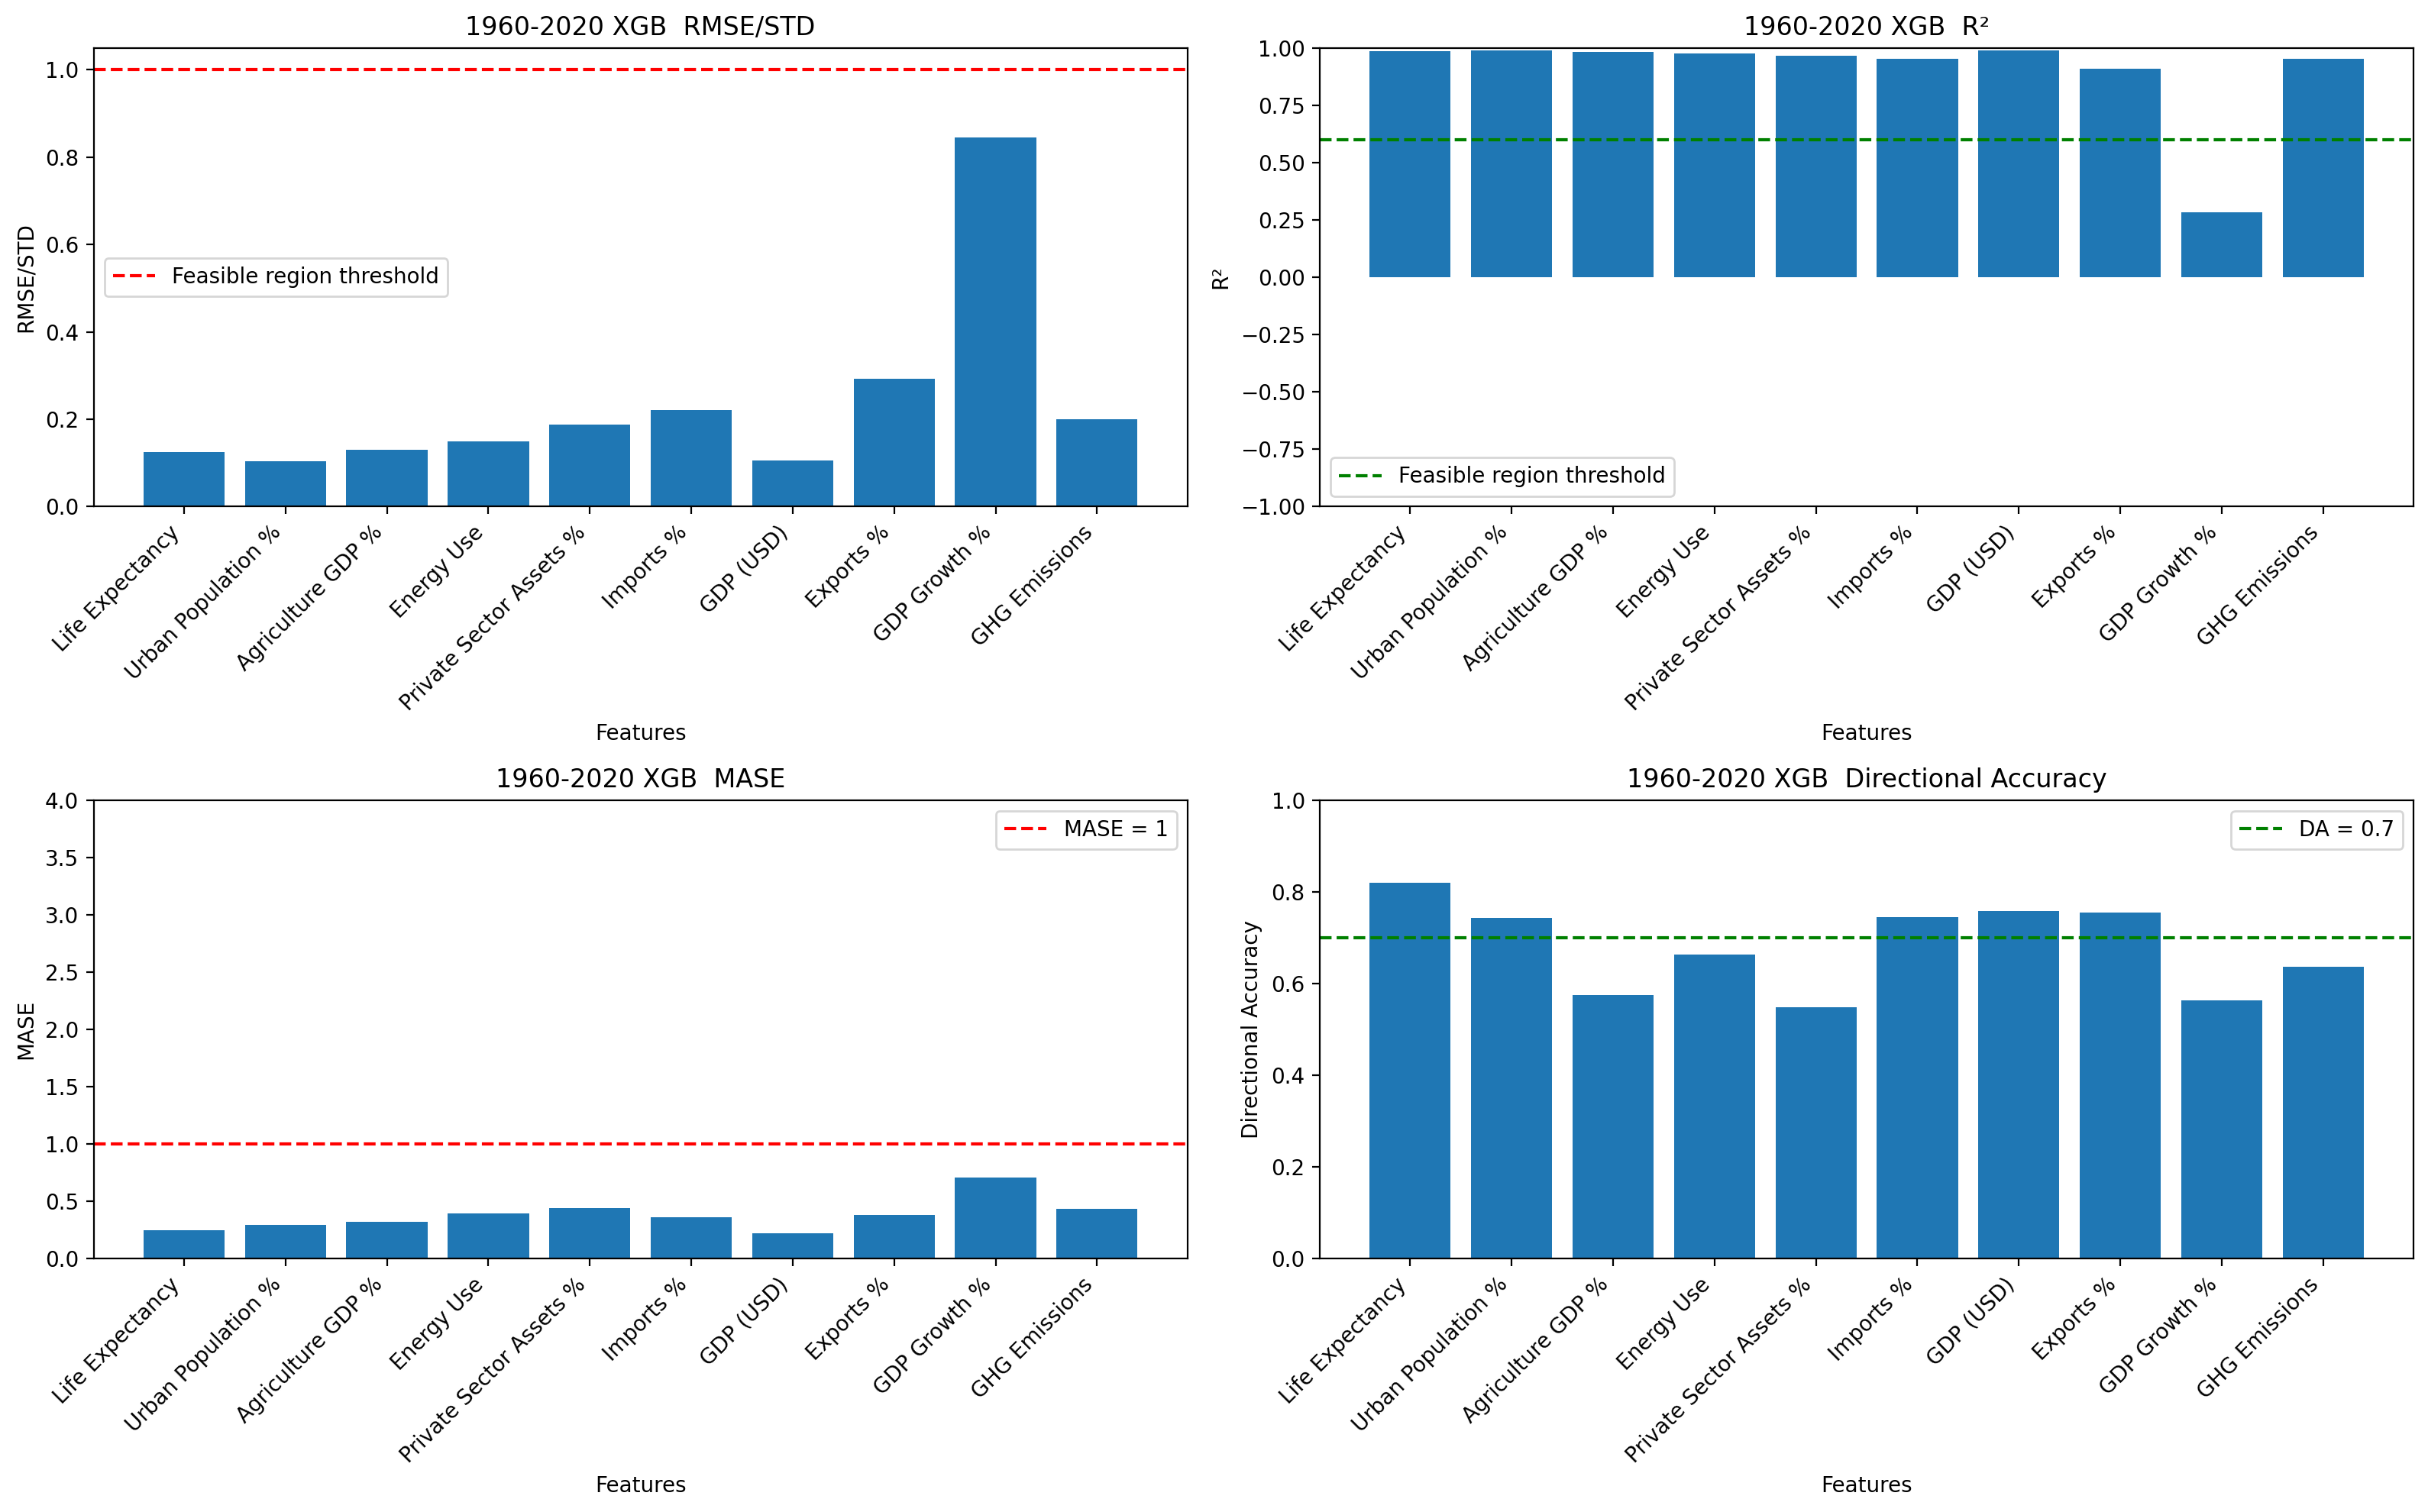
\includegraphics[width=\textwidth]{1960_2020_XGB_metrics_basic.png}
    \caption{Prediction performance of XGBoost for each feature (1960--2020), including RMSE/STD, $R^2$, MASE, and Directional Accuracy.}
    \label{fig:xgb_feature_summary}
\end{figure}



From Figure~\ref{fig:model_compare_1} and Figure~\ref{fig:model_compare_2}, We can divide the chosen Machine Learning algorithms into 3 different categories: 
\begin{itemize}
\item RF and XGB have best performances, both of which has a low standardized error, MASE and high $R^2$ and DA, with a guiding score over 2.5
\item LR, Ridge, Lasso, ElasticNet have very similar performances, with a guiding score about 2.0 (2010-2020)
\item LWR, SVR, KNN have comparatively low performances. This is in part because the sample size (M = 1220 or 220) is rather small compared to input features (N = 10)
\end{itemize}
Figure~\ref{fig:xgb_feature_summary} summarizes the prediction performance of XGBoost for each of the 10 selected indicators over the full period (1960--2020). The results indicate that XGBoost achieves high accuracy for most structural indicators, with standardized errors (RMSE/STD) well below 1 and $R^2$ values typically above 0.6. Notably, indicators such as life expectancy, urban population share, and energy use are predicted with particularly high precision. In contrast, GDP growth (annual \%) stands out as the only indicator with consistently poor predictive performance, exhibiting both high error and low explanatory power. The poor predictability of the GDP growth rate compared to other major indicators is primarily due to its intrinsic volatility, exposure to a broad set of unobserved influences, and its weak contemporaneous linkages with slow-moving structural features. This is a well-documented phenomenon in economic modeling ~\cite{Loungani2001, ClementsHendry2002}, where forecasting economic growth remains an exceptionally challenging task.


\subsection{Hyperparameter Tuning for XGBoost and Random Forest}

To ensure robust performance from the ensemble models, we conducted hyperparameter tuning for both XGBoost (XGB) and Random Forest (RF) using grid search with 5-fold cross-validation.

For XGBoost, the primary hyperparameters adjusted include:
\begin{itemize}
    \item \texttt{n\_estimators}: Number of boosting rounds.
    \item \texttt{max\_depth}: Maximum depth of each tree.
    \item \texttt{learning\_rate}: Step size shrinkage used in updates.
    \item \texttt{subsample}: Fraction of observations to be randomly sampled for each tree.
    \item \texttt{colsample\_bytree}: Fraction of columns to be randomly sampled for each tree.
\end{itemize}

For Random Forest, the tuning focused on:
\begin{itemize}
    \item \texttt{n\_estimators}: Number of trees in the forest.
    \item \texttt{max\_depth}: Maximum depth of the tree.
    \item \texttt{min\_samples\_split}: Minimum number of samples required to split an internal node.
    \item \texttt{max\_features}: Number of features to consider when looking for the best split.
\end{itemize}
\begin{figure}[h]
    \centering
    \begin{subfigure}[t]{0.9\textwidth}
        \centering
        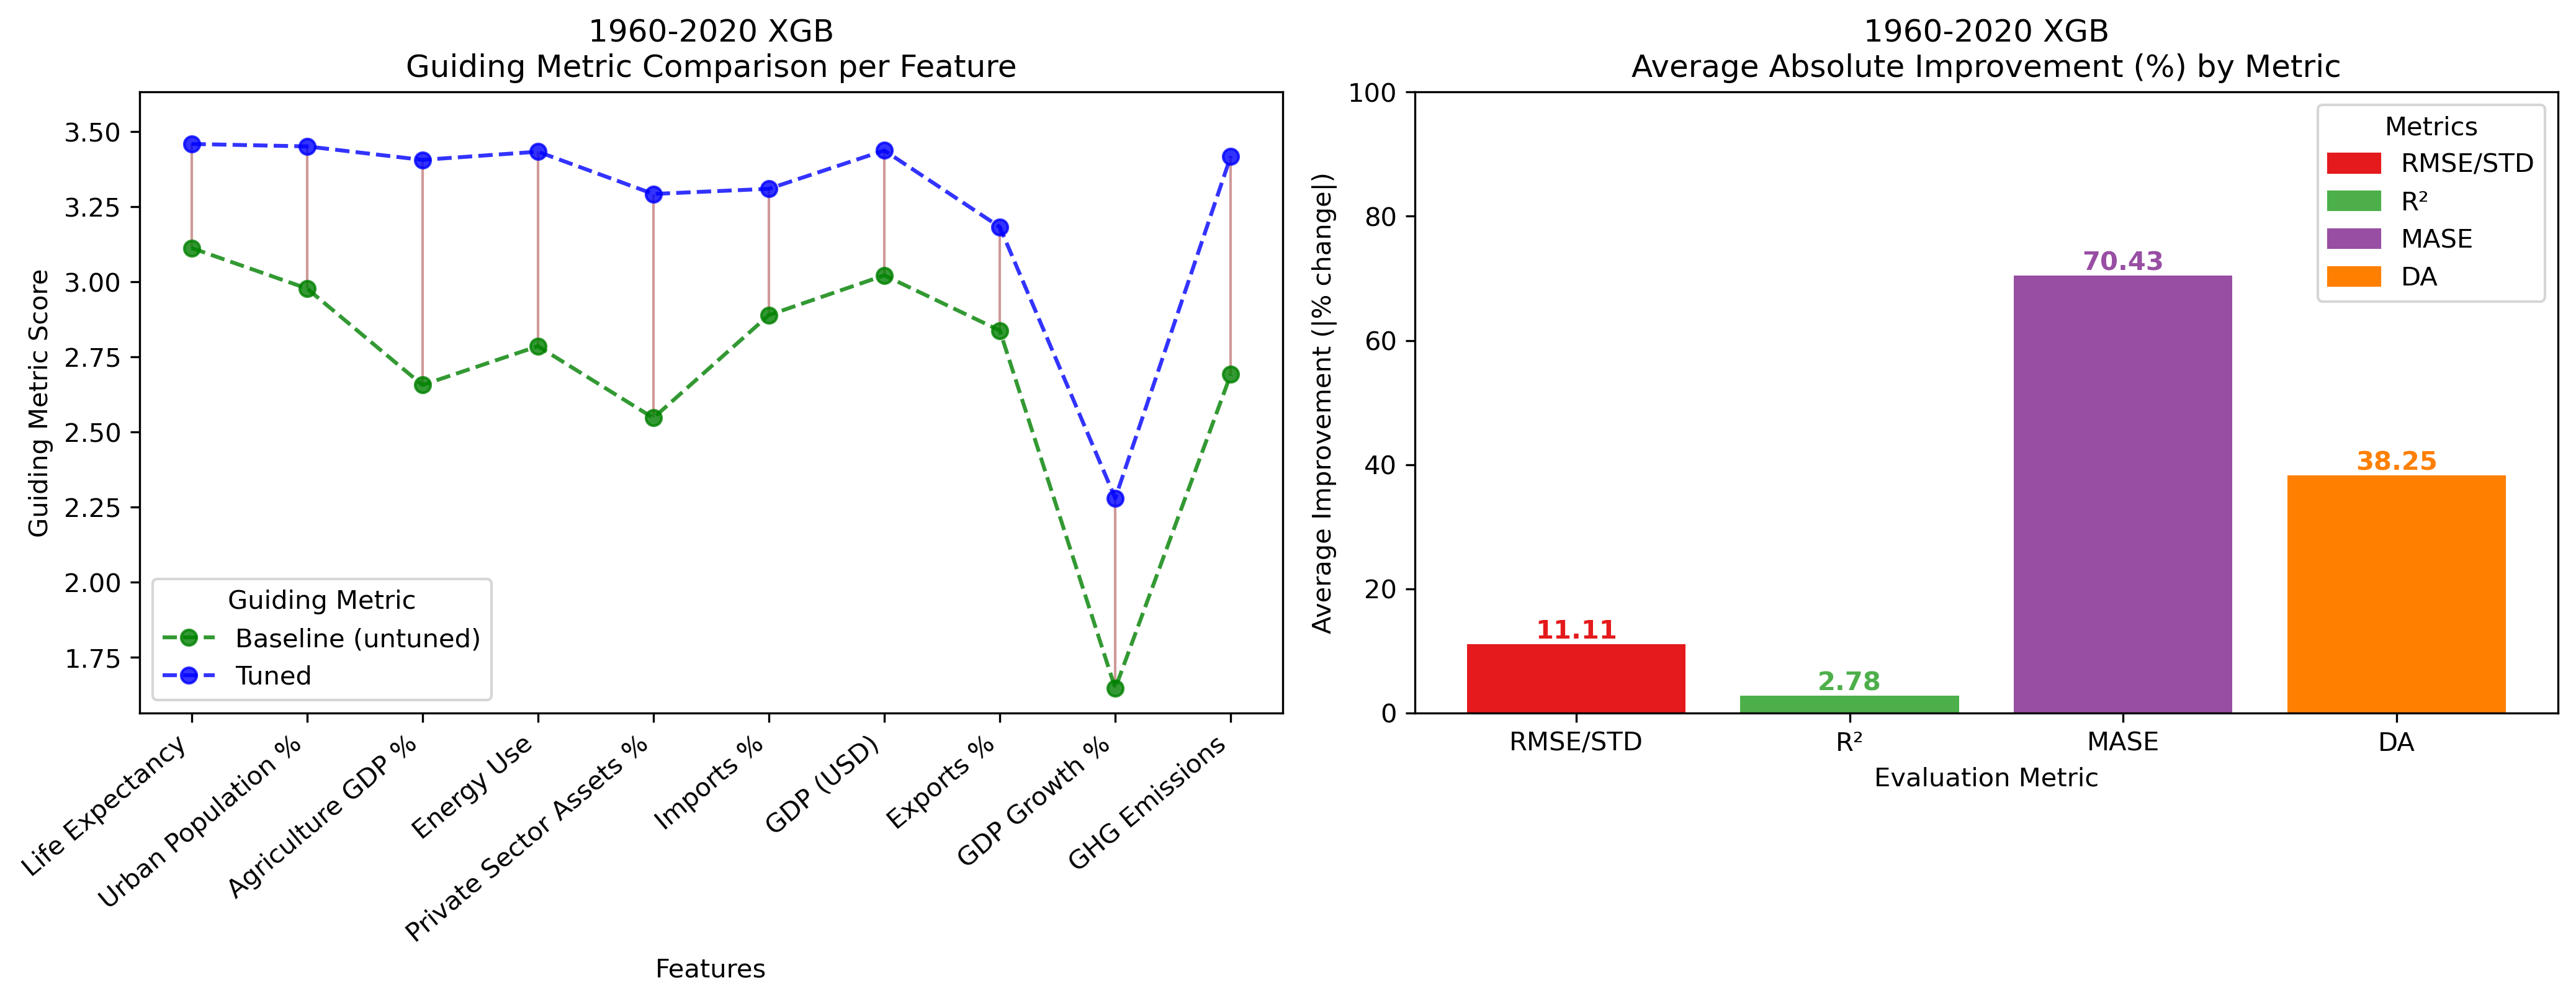
\includegraphics[width=\linewidth]{1960_2020_XGB_metrics.png}
        \caption{XGBoost: Tuning Performance (1960--2020)}
        \label{fig:xgb_tuning_1960_2020}
    \end{subfigure}
    \vspace{1em}
    \begin{subfigure}[t]{0.9\textwidth}
        \centering
        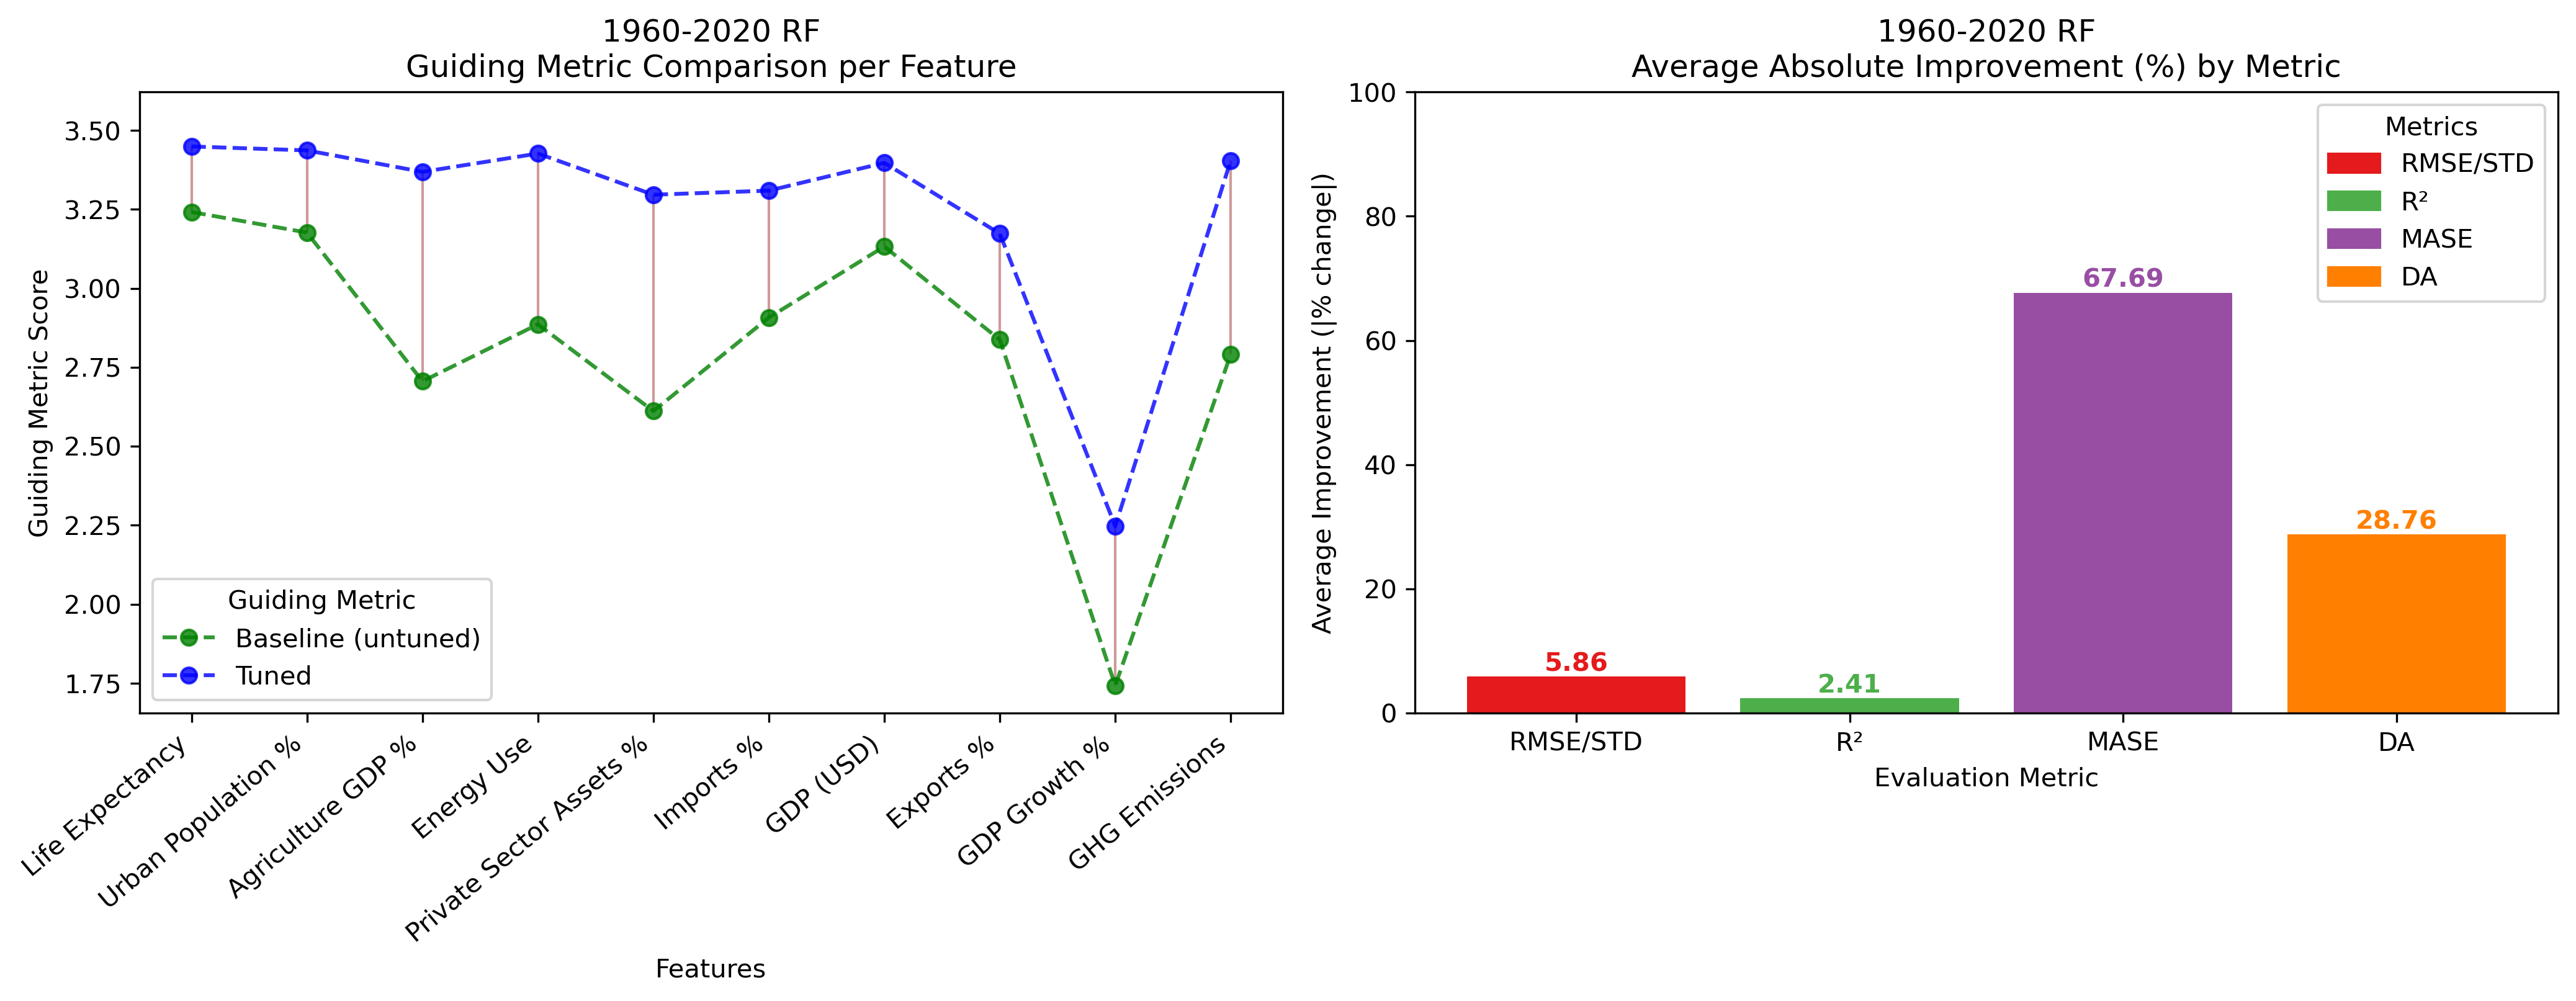
\includegraphics[width=\linewidth]{1960_2020_RF_metrics.png}
        \caption{Random Forest: Tuning Performance (1960--2020)}
        \label{fig:rf_tuning_1960_2020}
    \end{subfigure}
    \caption{Comparison of Hyperparameter Tuning Effects for XGBoost and Random Forest (1960--2020)}
    \label{fig:tuning_combined}
\end{figure}
Figure~\ref{fig:tuning_combined} illustrates how hyperparameter tuning improves model performance. Across all indicators, XGBoost consistently outperforms Random Forest, and both models benefit significantly from tuning.

Metric-wise, the most notable improvements appear in Directional Accuracy (DA), which rises by 30--40\%. This suggests that tuning not only improves numerical accuracy but also strengthens the models' ability to correctly predict the direction of change—a crucial feature for real-world policy and decision-making. Improvements in RMSE/STD and MASE are also evident, especially for structural indicators. In contrast, $R^2$ gains are modest, indicating that tuning has limited effect on variance explanation but substantial effect on practical usability.

Overall, tuning contributes most to directional consistency and error reduction, making ensemble models more robust and interpretable across diverse indicators.

Figure~\ref{fig:tuning_combined} provides a detailed visualization of the performance improvements after tuning. The left panel illustrates that while the magnitude of improvement of guiding score varies across indicators, all ten features experience a substantial average enhancement. This confirms that tuning has universal benefit, though its effect size depends on feature characteristics.

The right panel decomposes improvements across the four evaluation metrics. Notably, tuning yields minimal changes in $R^2$ (near 2\%), modest gains in RMSE/STD (ranging from 5\% to 10\%), and substantial improvements in Directional Accuracy (DA), which increase by approximately 30\%--40\%. The most dramatic effect is observed in Mean Absolute Scaled Error (MASE), where XGBoost and Random Forest achieves a nearly 70\% improvement. 
These results highlight how hyperparameter tuning differentially impacts specific model objectives and offer insights into which dimensions of forecast accuracy are most tunable.

\subsection{Summary}

Chapter 4 evaluated the feasibility of cross-indicator forecasting using machine learning models applied to national-level economic and social data. By predicting each indicator from the remaining features, we tested nine models across two time periods (1960–2020 and 2010–2020), and evaluated their performance using a composite guiding score.

XGBoost and Random Forest consistently outperformed other models, supporting the broader literature on the strengths of ensemble methods in capturing nonlinear macroeconomic patterns~\cite{Mullainathan2017ML, Athey2019ML}. Structural indicators—such as life expectancy, urban population, and energy use—were highly predictable, showing low error and strong directional accuracy. In contrast, GDP growth remained inherently difficult to forecast due to volatility and external shocks~\cite{Loungani2001, ClementsHendry2002}.

Model performance also improved in the 2010–2020 window, likely reflecting better data quality and macroeconomic convergence across countries~\cite{Baldwin2016Great, Jerven2013Poor}. These results emphasize the importance of model type, indicator stability, and temporal context in determining forecast reliability.

In summary, ensemble-based machine learning models, when properly tuned and evaluated with a balanced metric like the guiding score, offer a robust framework for forecasting slow-moving national indicators. This lays a solid foundation for the time-series and cross-national forecasting explored in subsequent chapters.


\section{Country-Level Time Series Forecasting}


\subsection{Dataset and Feature Construction}

This chapter uses the same interpolated dataset from 1960 to 2020 as in Chapter 4, including all available countries. For each of the 10 selected key indicators, we constructed lag-based time series features to facilitate temporal prediction modeling. Specifically, we created lag-2 and lag-3 versions of all other features (excluding the target) to predict each target feature value year by year.

The resulting time series dataset preserves the year and country code metadata, and ensures that the predictive modeling process incorporates temporal dynamics. All features were standardized prior to modeling to avoid scale issues.

\subsection{Models and Design Logic}

We evaluated six models for each country and each target indicator:

\begin{itemize}
    \item \textbf{Naive Forecast}: Uses the value of the previous year as the prediction for the next year.
    \item \textbf{ARIMA}: A univariate autoregressive model applied independently to each target series.
    \item \textbf{XGB-lag2}: A gradient-boosted decision tree using lag-2 features of all other variables to predict the target.
    \item \textbf{XGB-lag3}: Similar to the above, but with lag-3 features.
    \item \textbf{Rolling XGB-lag2}: Same as XGB-lag2, but predictions are generated year-by-year using only prior data up to that year (rolling forecast).
    \item \textbf{Rolling XGB-lag3}: Extends the rolling forecast logic to lag-3 input features.
\end{itemize}

The rolling forecast strategy better simulates real-world forecasting where future data is unavailable during training. The comparison across static and rolling variants allows us to evaluate model generalizability and robustness over time.

\subsection{Model Comparison}
% Compare forecasting performance of different time series models on a selected country.
% ------------------------------ Figure 6 Analysis ------------------------------
\subsubsection*{Country-Level Model Feasibility Analysis (Figure 6)}


\begin{figure}[H]
    \centering
    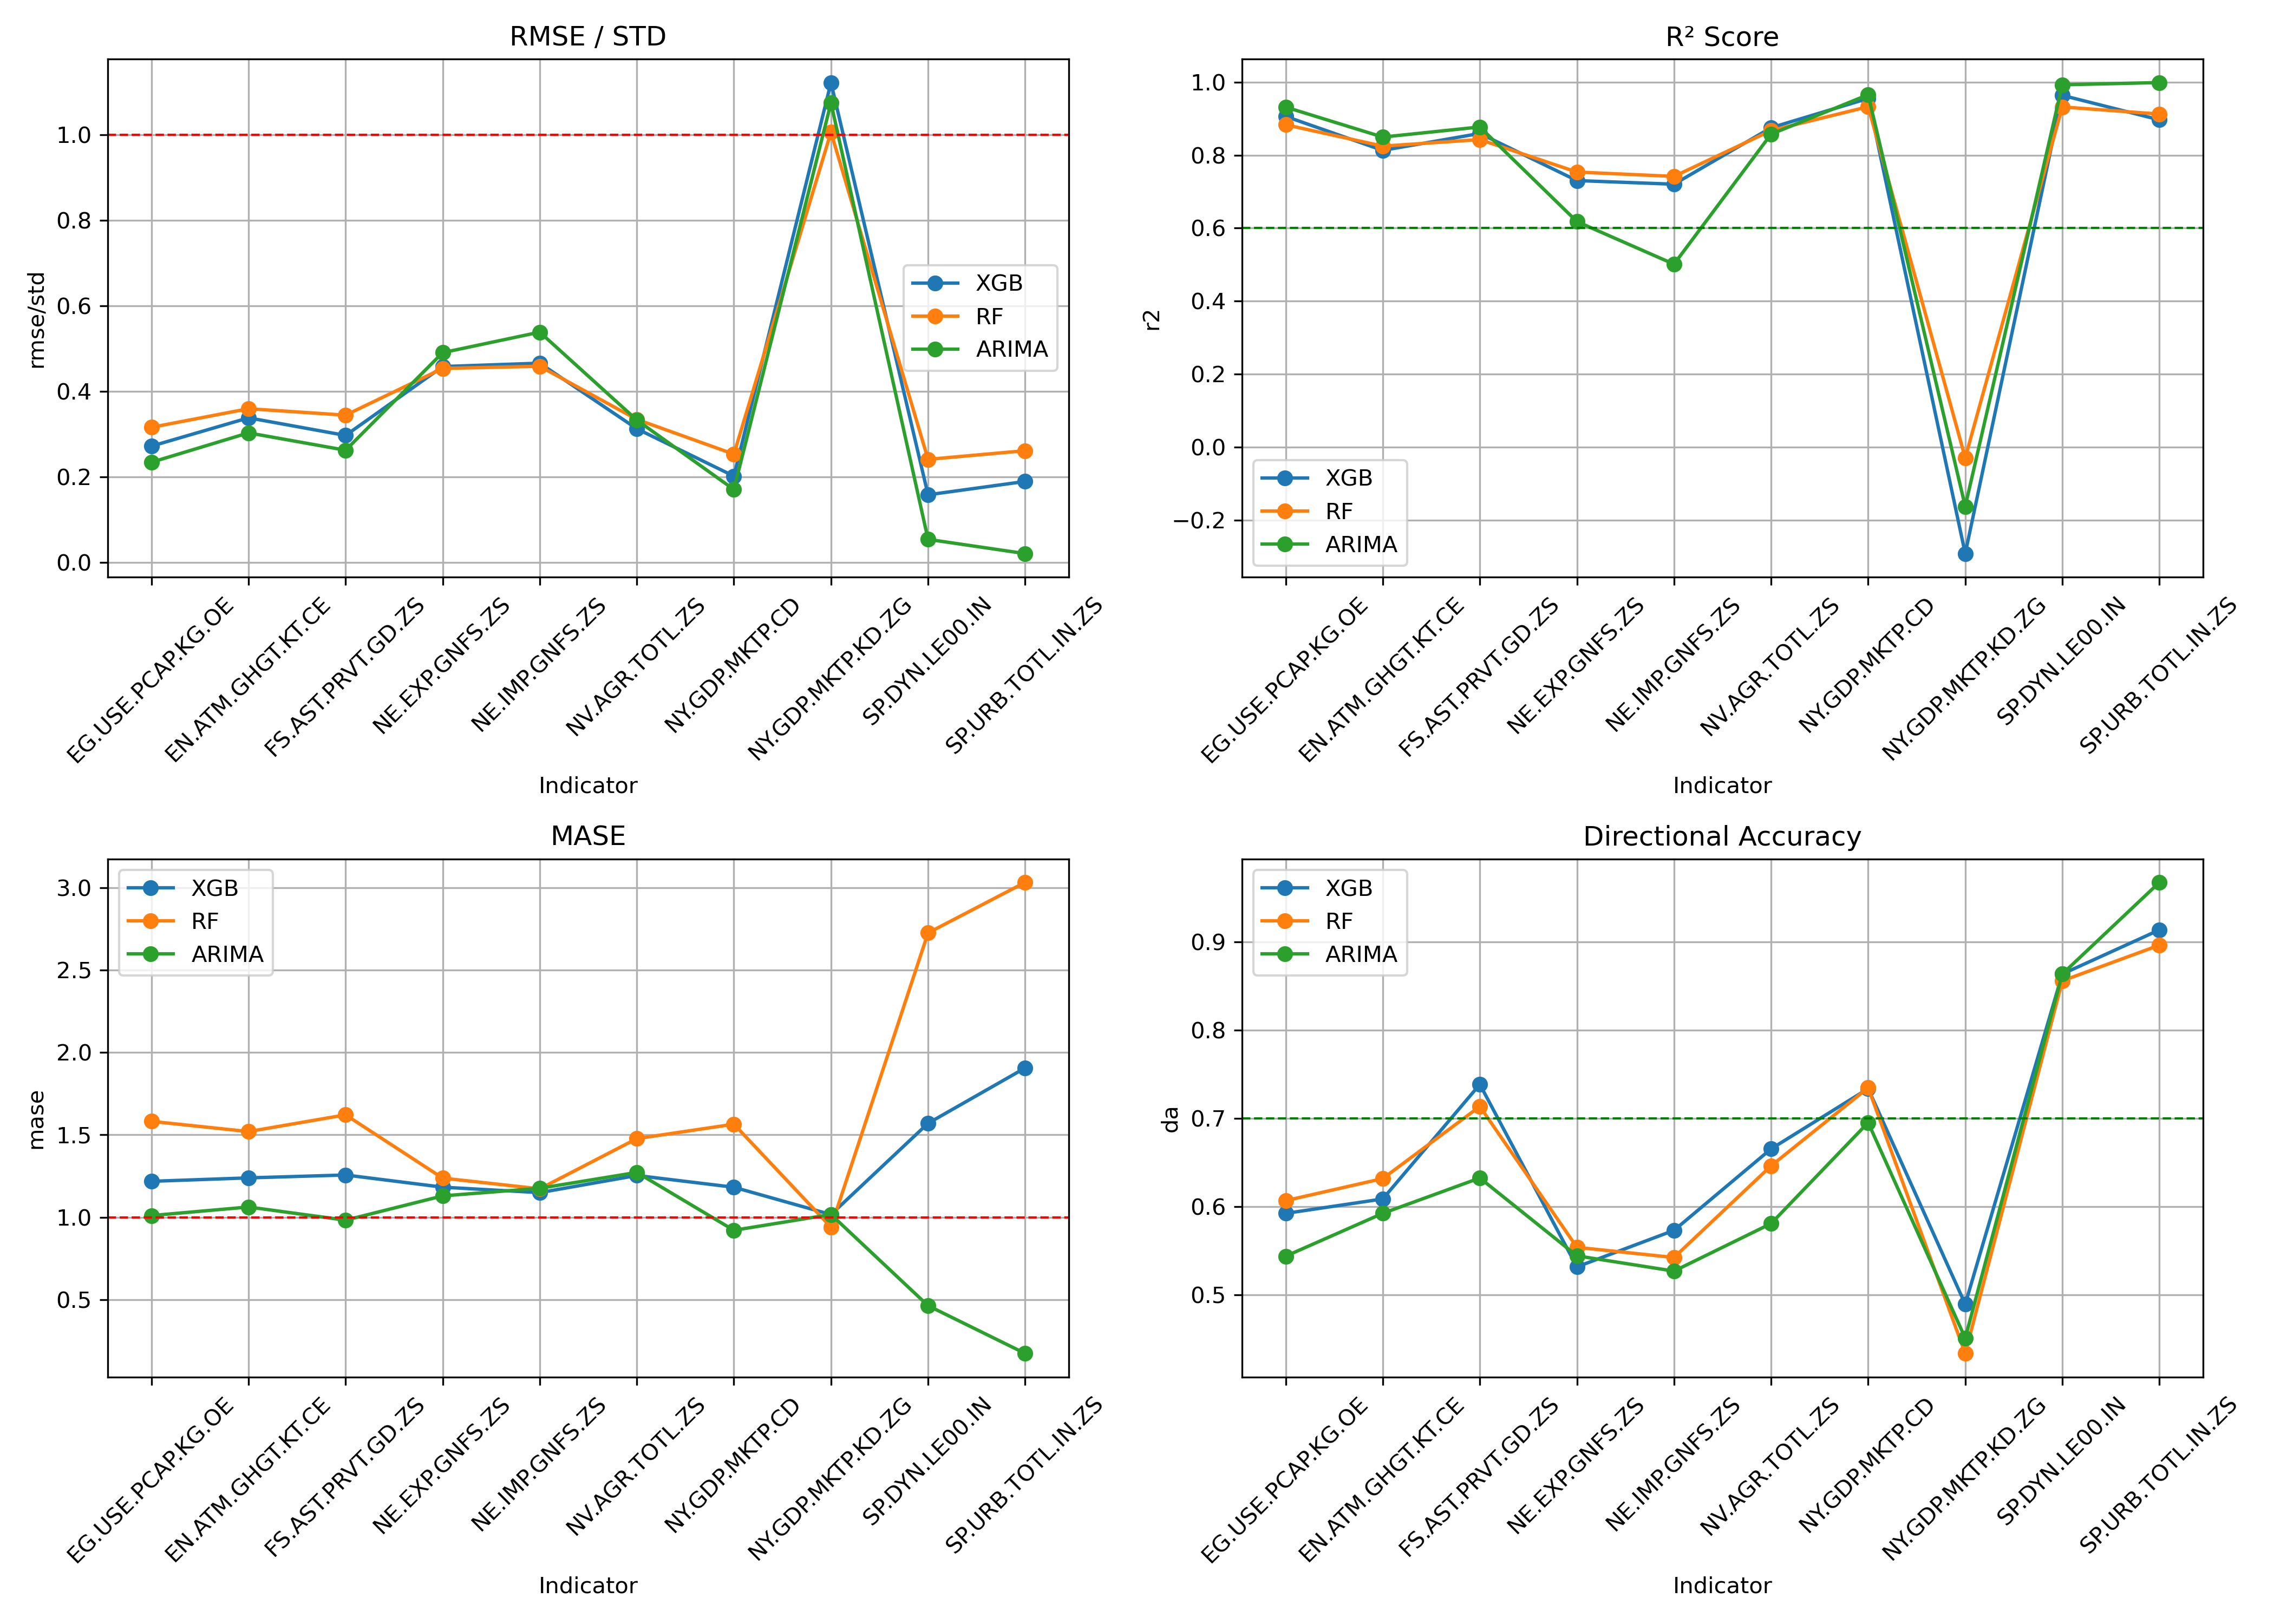
\includegraphics[width=\textwidth]{figure4.png}
    \caption{Comparison of model performance across indicators using four metrics: RMSE/STD, $R^2$, MASE, and Directional Accuracy (DA). }
    \label{fig:indicator_comparison}
\end{figure}

Figure~\ref{fig:indicator_comparison} visualizes the prediction performance of three time series models—XGBoost, Random Forest, and ARIMA—across ten selected macroeconomic indicators. Each subfigure corresponds to one of the four evaluation metrics, with threshold lines indicating feasibility standards.

Across most indicators, all three models achieve standardized errors (RMSE/STD) well below the cutoff of 1. The exception is GDP growth rate, where all models exhibit RMSE/STD above the threshold, confirming its inherent volatility and poor predictability again.

In terms of explanatory power ($R^2$), all three 
models perform strongly on indicators like life expectancy and GDP, often exceeding $R^2 = 0.9$. 
However, for GDP growth, the $R^2$ values drop dramatically, reaching negative values for all three models, reflecting their inability to explain variance in this highly unstable target. This result aligns with long-standing findings in the forecasting literature that GDP growth is notoriously difficult to predict due to its susceptibility to external shocks, technological shifts, and policy discontinuities \cite{Loungani2001, ClementsHendry2002}.

For MASE, ARIMA outperforms both XGBoost and RF on average, particularly for stable indicators like urban population share and life expectancy. However, it should be noted that MASE values for all models tend to exceed the benchmark threshold of 1 on volatile indicators such as GDP growth and trade-related variables. This suggests that while ARIMA benefits from its statistical simplicity, its absolute accuracy remains limited when faced with non-stationary or rapidly shifting macroeconomic environments \cite{Hyndman2006}.

In terms of Directional Accuracy (DA), indicators such as the assets of private sector banks to GDP and overall GDP exhibit strong predictive signals, with all three models achieving DA values above 0.7. Notably, life expectancy and urban population rate emerge as the most directionally stable indicators, with ARIMA approaching near-perfect DA on urbanization—a phenomenon likely driven by the smooth, monotonic trajectories of demographic transitions \cite{Bloom2008, Montgomery2003}. These findings indicate that structural indicators with persistent trends are well suited to directional prediction, even by relatively simple models.

Overall, the heatmap illustrates that while machine learning and statistical models can robustly capture long-term structural patterns, their performance deteriorates on high-volatility targets like GDP growth. This reinforces the need for volatility-aware modeling strategies and careful consideration of economic context when selecting forecast targets.

% ------------------------------ Figure 7 Analysis ------------------------------
\subsubsection*{Indicator-Specific Feasibility by Country (Figure 7)}


\begin{figure}[h]
    \centering
    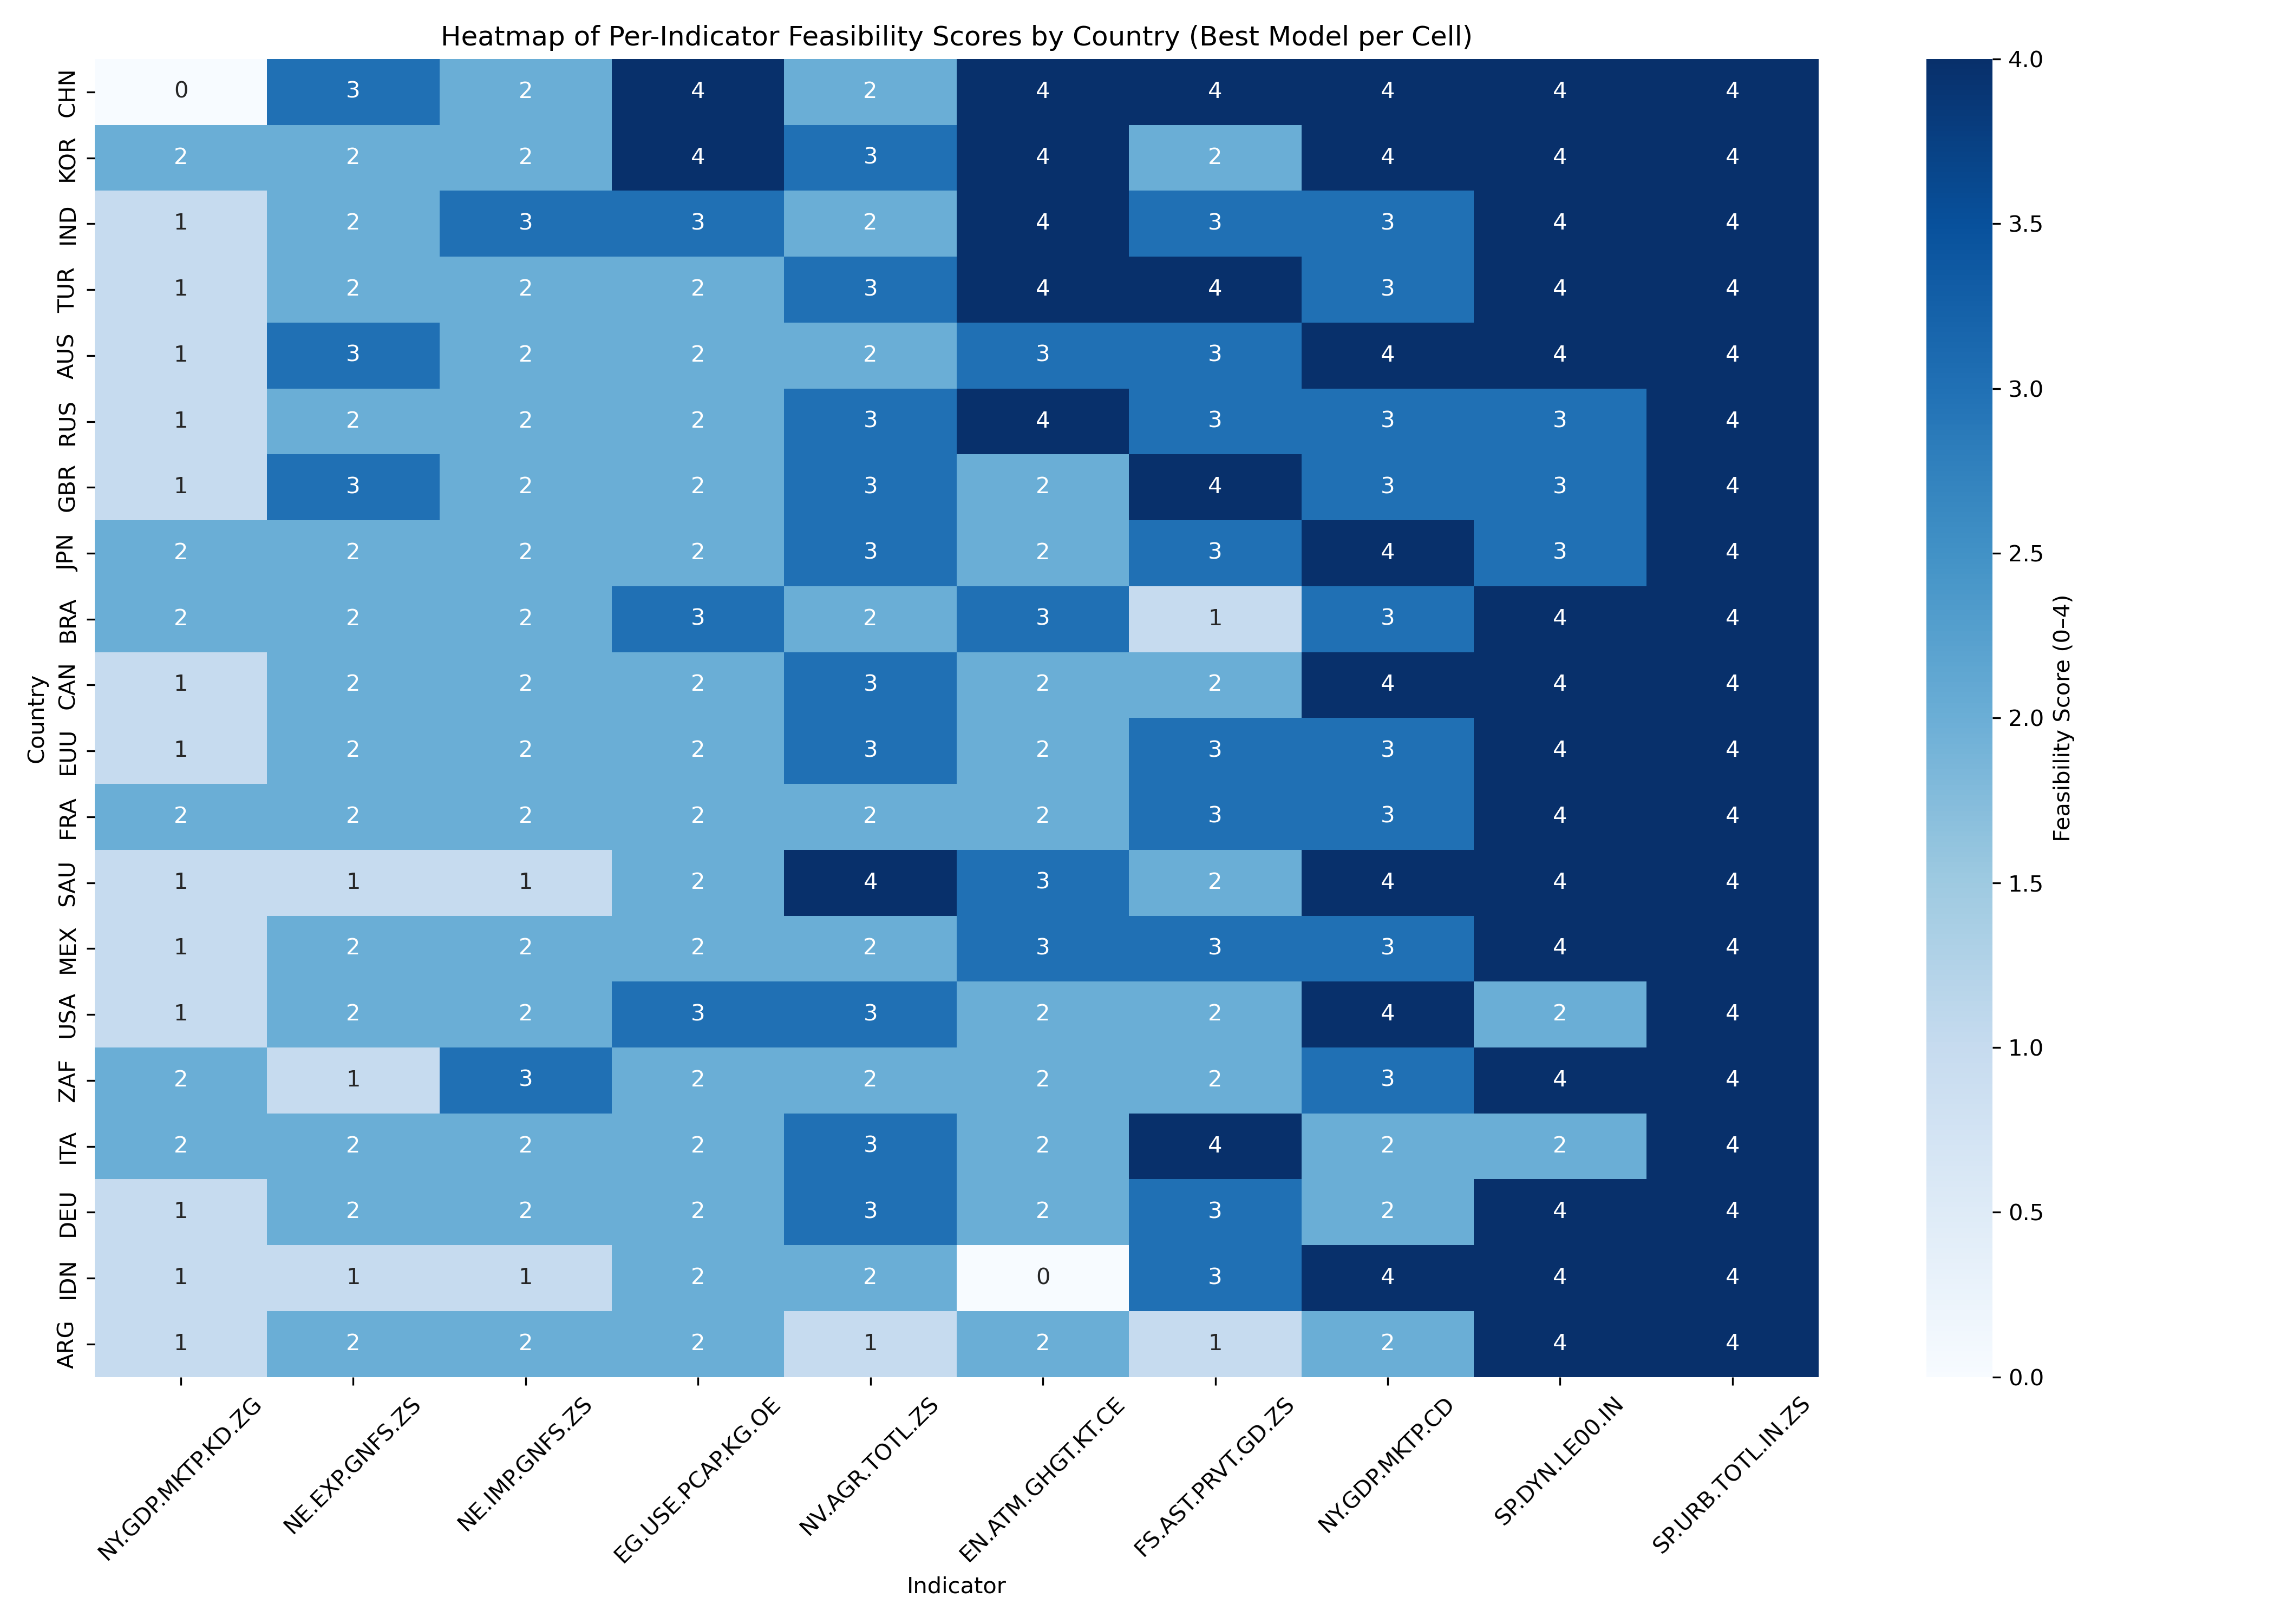
\includegraphics[width=\textwidth]{figure8.png}
    \caption{Heatmap of Per-Indicator Feasibility Scores by Country. For each (country, indicator) pair, we select the best-performing model and report the corresponding feasibility score (0–4). Darker colors indicate more reliable prediction.}
    \label{fig:heatmap_feasibility}
\end{figure}


Figure~\ref{fig:heatmap_feasibility} visualizes the feasibility of predicting macroeconomic indicators across countries using their respective best-performing models. Each cell represents the maximum feasibility score (out of 4)\footnote{For a certain (Country, Model, Indicator), feasbility rate is the sum of $\alpha_i$'s. We have chosen the best model for each (Country, Indicator)} attained by any model for a given (country, indicator) pair. The darker the cell, the higher the reliability of the forecasted value according to our composite metric that combines RMSE/STD, $R^2$, MASE, and Directional Accuracy (DA).

Several key insights emerge:

First, countries such as China, Korea, and India consistently exhibit high feasibility scores across nearly all indicators. Their rows are dominated by the darkest shades, indicating that for these countries, most structural indicators can be predicted with high reliability. This may reflect the availability of cleaner, more complete data, along with stable structural development patterns in these emerging economies \cite{Chen2011development, OECD2019india}.

In contrast, countries such as Argentina, Denmark, and Italy show a wider variance in feasibility across indicators, with many scores clustered around 1–2. This suggests higher volatility or data inconsistency, which impairs model effectiveness even when choosing the best available model.

Second, certain indicators are predictably easier across the board. Urban population\%, life expectancy, and GDP display high scores for almost all countries. These features represent slow-moving structural trends that evolve gradually over time, enabling models to capture their trajectories effectively regardless of the country context.

In contrast, GDP growth\% and trade-related indicators are challenging to predict for most countries, with many feasibility scores below 2. This aligns with findings in forecasting literature that highlight the unpredictability of growth due to sensitivity to shocks, policy regime changes, and latent external factors \cite{Loungani2001, ClementsHendry2002}.

Finally, the heatmap also demonstrates the value of a model-selection strategy. By selecting the best-performing model per cell rather than applying a single model globally, we are able to surface reliable predictions even in challenging data regions. This justifies the use of hybrid or adaptive pipelines in global macroeconomic forecasting tasks.

These results highlight that the feasibility of economic forecasting is a function not only of algorithmic design, but also of indicator volatility, national structural consistency, and the flexibility of the modeling pipeline.
\subsection{Case Study: China}

To ground our analysis in a concrete national context, we present a case study on China—an economy that demonstrates consistently high feasibility scores across indicators. Figure~\ref{fig:china_ts_metrics} summarizes the rolling forecast performance of three models (XGBoost, Random Forest, and ARIMA) across four evaluation metrics for ten selected indicators.

\begin{figure}[H]
    \centering
    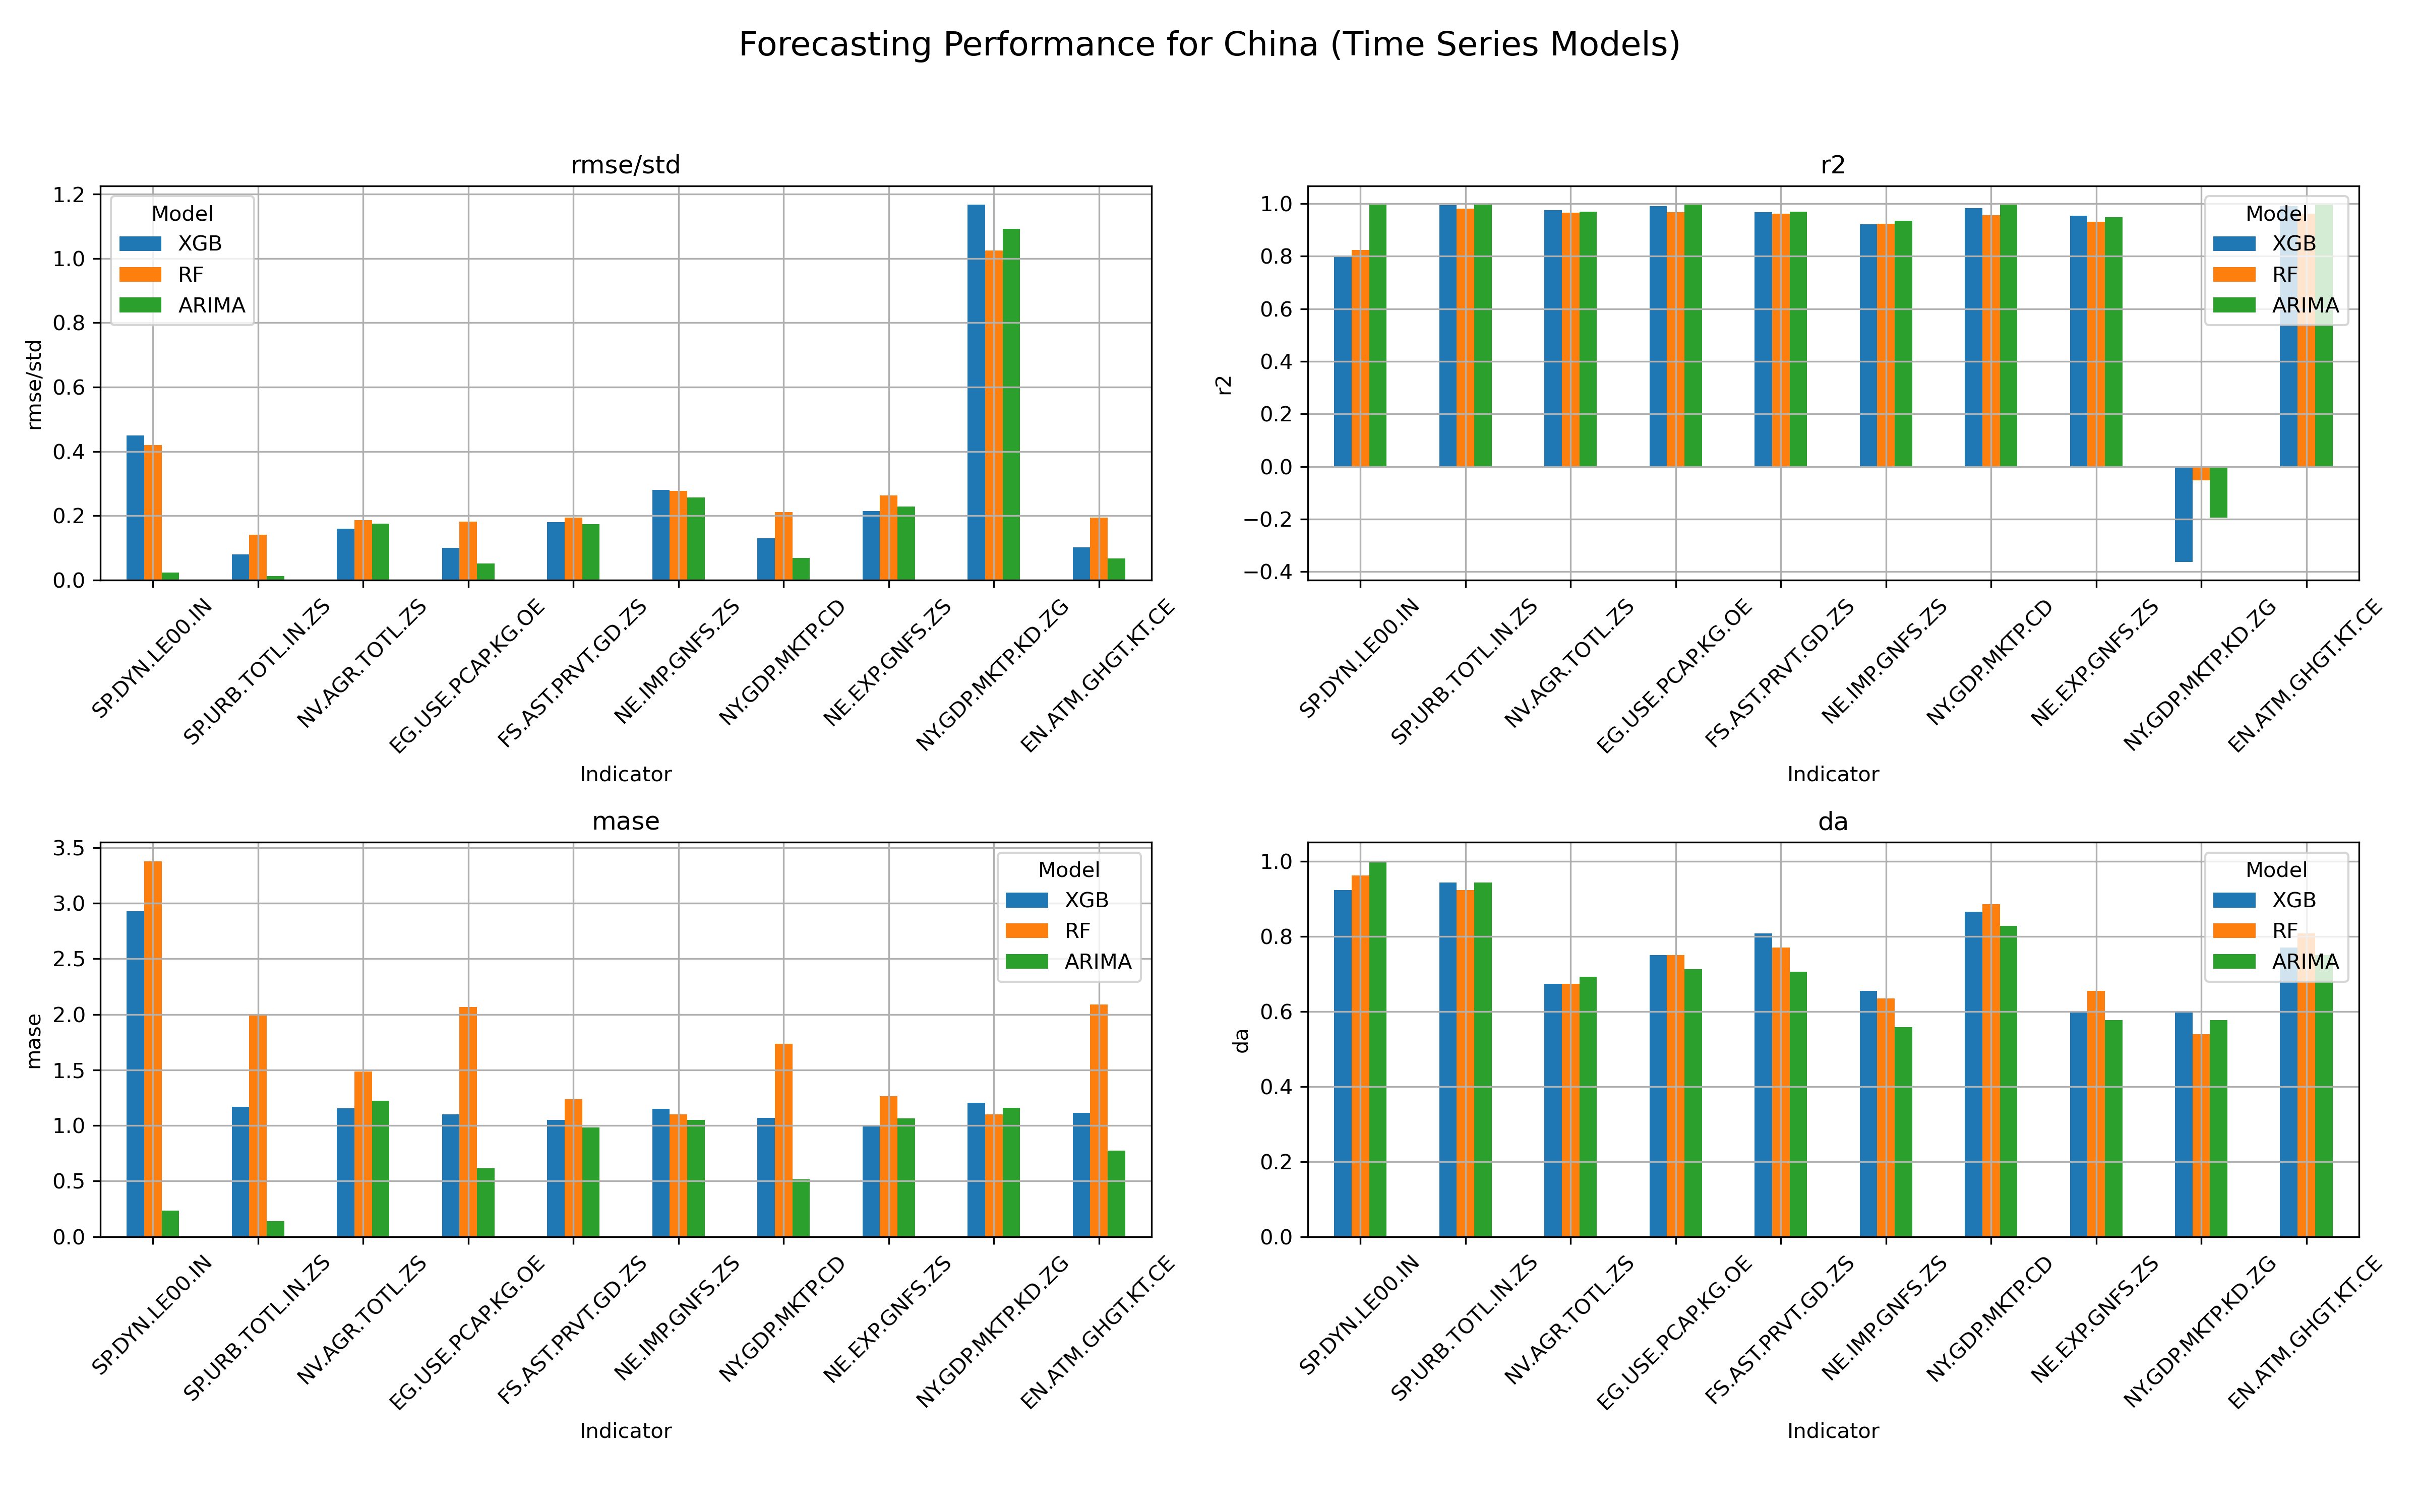
\includegraphics[width=\textwidth]{china_case_comparison.png}
    \caption{Model performance for China across ten indicators and four evaluation metrics.}
    \label{fig:china_ts_metrics}
\end{figure}

Across all metrics, China's performance aligns with our broader findings. Indicators such as life expectancy, urban population\%, and energy use show excellent predictability, with RMSE/STD values below 0.2, $R^2$ scores near or above 0.9, and Directional Accuracy (DA) values nearing 1. ARIMA exhibits particularly strong DA and MASE performance on stable, trend-dominated indicators, consistent with its statistical strengths.

However, GDP growth once again resists accurate modeling: all three models produce negative $R^2$ and high MASE, confirming its structural volatility. Interestingly, XGBoost performs slightly better than ARIMA and RF on most indicators in RMSE and $R^2$, although ARIMA sometimes surpasses machine learning models in DA and MASE on low-variance series.

This case study confirms China's suitability for time-series forecasting using machine learning, due to its consistent long-run development patterns and high-quality data.\cite{zhang2020china, xie2018macroeconomic} It also reinforces our earlier conclusion that indicator characteristics—such as structural stability—matter more than country size or development stage in determining forecast feasibility.
\subsection{Case Study: United States}

To provide a comparative benchmark to China, we analyze forecasting performance in the United States (US)—a developed economy with high data availability but greater macroeconomic volatility. Figure~\ref{fig:us_ts_metrics} summarizes results for the same set of indicators and models.

\begin{figure}[H]
    \centering
    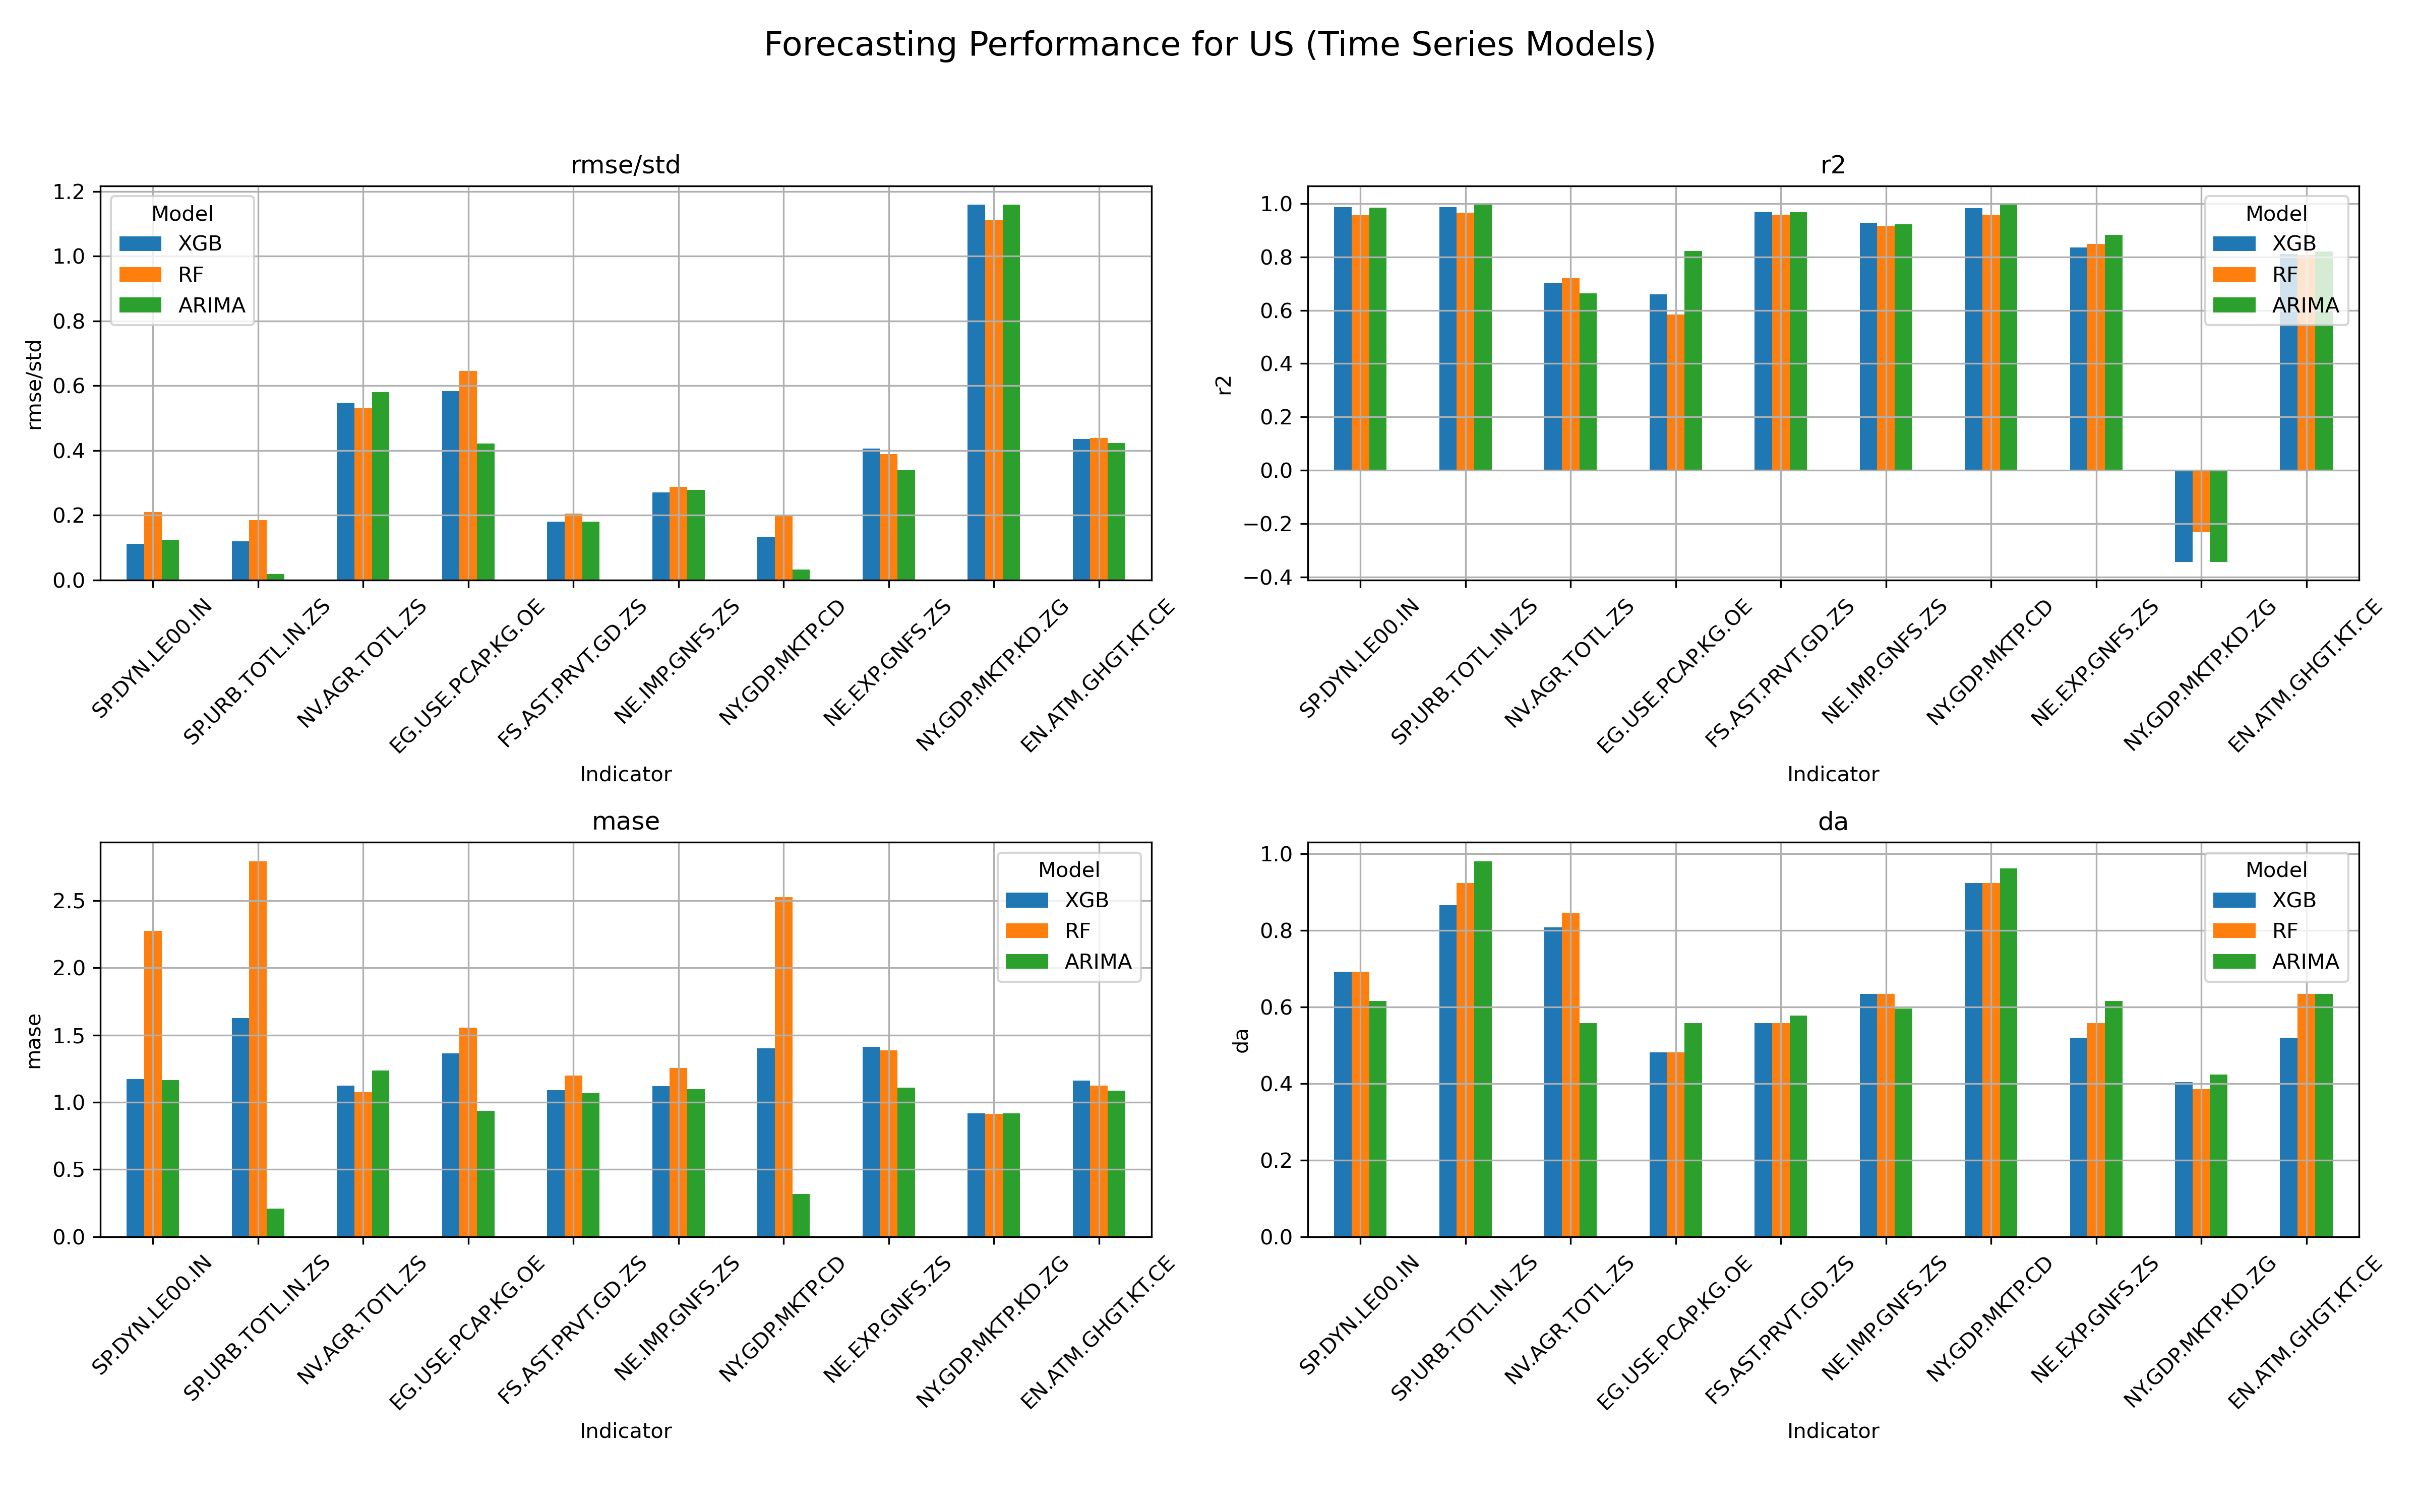
\includegraphics[width=\textwidth]{us_case_comparison.png}
    \caption{Model performance for the United States across ten indicators and four evaluation metrics.}
    \label{fig:us_ts_metrics}
\end{figure}

The US results reveal several notable contrasts. While indicators such as urban population share and energy use remain highly predictable (RMSE/STD $<$ 0.2, $R^2 > 0.9$), other indicators—such as private sector assets and import/export ratios—show more erratic performance. This is particularly evident in MASE and DA, where RF performs poorly and exhibits higher variability.

GDP growth remains the least predictable, with negative $R^2$ and MASE above 1 across all models, echoing global trends. However, ARIMA outperforms XGBoost and RF on several indicators, especially in DA and MASE for urbanization and energy use, likely due to the smoother underlying dynamics and higher data quality.

Interestingly, while XGBoost retains a slight edge in RMSE and $R^2$ for several features, its gains over ARIMA are marginal in stable indicators and its performance deteriorates in the presence of high-frequency noise. This suggests that, in the US context, statistical models remain competitive for long-term indicators, but ensemble ML models show more robustness to mid-range structural variation.

\subsubsection*{Comparison: China vs. United States}

The China-US comparison highlights that strong performance depends not only on model choice but also on data structure and volatility. China's indicators tend to follow smoother trajectories—perhaps due to stronger long-term policy continuity and structural reforms—making them more amenable to both ML and statistical forecasting. In contrast, the US exhibits more structural breaks and market-driven fluctuations, reducing feasibility rates for some indicators.\cite{stock2002structural, koop2013us}

Despite these differences, both countries achieve strong predictability on structural features like life expectancy, urbanization, and energy use. These shared patterns suggest that for these indicators, cross-national model generalization may be viable. Conversely, volatility-sensitive indicators such as GDP growth, trade shares, and financial ratios remain country-specific in their forecasting challenges.

Overall, this comparative case study reinforces the earlier conclusion that temporal predictability is not solely a function of economic development level, but of indicator-specific dynamics and national structural stability.\cite{lin2012newstructural, reifschneider2015usforecasting}
\subsection{Discussion}

The country-level time series analysis presented in Sections 5.1–5.5 reveals several critical insights into the nature of temporal predictability in macroeconomic indicators.

First, certain indicators—such as life expectancy, urbanization, and energy use—consistently demonstrate strong forecast performance across all countries and models. Their trajectories are largely monotonic and driven by structural factors such as demographic transition, urban planning, and industrialization. As such, they lend themselves well to both statistical models like ARIMA and machine learning models such as XGBoost and Random Forest. This supports previous findings that long-run demographic and energy trends are highly forecastable due to their persistence and data quality \cite{Bloom2008, xie2018macroeconomic}.

Second, GDP growth and trade-related variables remain inherently difficult to forecast, showing high MASE and low or negative $R^2$ across countries. This reinforces the broader literature that stresses the unpredictability of short-run economic performance due to the influence of external shocks, geopolitical disruptions, and endogenous cycles \cite{Loungani2001, stock2002structural}. Even sophisticated models cannot reliably capture the turning points or volatility associated with these indicators, especially when relying solely on autoregressive features.

Third, cross-country differences play a notable role. Emerging economies like China and India tend to exhibit smoother transitions in structural indicators, likely due to long-term policy planning and investment-driven growth patterns \cite{zhang2020china, OECD2019india}. In contrast, advanced economies such as the United States experience more frequent structural breaks and cyclical volatility, resulting in uneven model performance across indicators.

Fourth, the feasibility heatmap reveals the importance of adaptive model selection. By dynamically choosing the best-performing model for each country-indicator pair, we achieve significantly higher reliability than any single-model approach. This result underscores the heterogeneity of temporal dynamics across countries and indicators and supports the development of hybrid forecasting pipelines.

Lastly, the consistent performance of ARIMA on directionally stable indicators suggests that simple statistical baselines should not be overlooked. While machine learning models dominate in terms of scale-sensitive metrics (RMSE, $R^2$), ARIMA often outperforms them in directional accuracy and robustness, particularly in low-variance contexts.

These findings reinforce the value of a mixed-methods approach and highlight the complementarity between machine learning and traditional statistical techniques in macroeconomic forecasting.

\subsection{Hyperparameter Tuning for XGBoost, Random Forest}

% --- Begin Chapter 6 ---
\section{Chapter 6: Cross-Country Temporal Forecasting}


\subsection{Modeling Setup}
% Define time alignment across countries. Optional: DTW similarity, cross-country lagged features.

\subsection{Cross-National Forecasting}
% Analyze how models trained on one or multiple countries generalize to others.

\subsection{Trend and Volatility Analysis}
% Identify persistent temporal trends vs high-volatility indicators across countries.

\subsection{Discussion}
% Reflect on structural similarity, transferable patterns, and policy relevance of findings.

\section{Conclusion}

This work demonstrates that most major structural indicators of national development are highly predictable from a small set of other key indicators, especially when using ensemble tree-based machine learning models. The exception is GDP growth rate, which remains notoriously difficult to forecast—consistent with macroeconomic theory and previous empirical research.

Our results suggest that, for long-run cross-country comparative analysis, reliable prediction of most economic and demographic indicators is feasible using standard machine learning approaches and open-access datasets. However, caution should be exercised when interpreting models for inherently volatile outcomes such as economic growth. Overall, this study highlights the promise and limitations of data-driven prediction in international development research and points to several avenues for further methodological and substantive refinement.


\section*{Project Repository}
The full code, data preprocessing scripts, and results can be found at: [GitHub link will be inserted here].



\bibliographystyle{unsrt}
\bibliography{references}
\end{document}